%%%%%%%%%%%%%%%%%%%%%%%%%%%%%%%%%%%%%%%%%%%%%%%%%%%%%%%%%%%%%%%%%%%%%%%%
%                                                                      %
%     File: Thesis_Introduction.tex                                    %
%     Tex Master: Thesis.tex                                           %
%                                                                      %
%     Author: Andre C. Marta                                           %
%     Last modified : 13 May 2019                                      %
%                                                                      %
%%%%%%%%%%%%%%%%%%%%%%%%%%%%%%%%%%%%%%%%%%%%%%%%%%%%%%%%%%%%%%%%%%%%%%%%

\chapter{Introduction}
\label{chapter:introduction}

%%%%%%%%%%%%%%%%%%%%%%%%%%%%%%%%%%%%%%%%%%%%%%%%%%%%%%%%%%%%%%%%%%%%%%%%
\section{Motivation}
\label{section:motivation}

General relativity, developed by Albert Einstein, is a comprehensive theory of gravitation that fundamentally alters our understanding of the force of gravity. It portrays gravity not as a Newtonian force, but rather as a consequence of the curvature of spacetime caused by the presence of mass and energy. According to this theory, objects move through spacetime along paths dictated by this curvature, giving rise to the illusion of gravitational force. \\

One intriguing prediction of general relativity is the existence of black holes, celestial objects with such immense gravitational pull that nothing, not even light, can escape their grasp. In the context of general relativity, the presence of a black hole causes spacetime to contort and deform, leading to bizarre phenomena like time dilation and the bending of light rays. To an observer located at a significant distance from a black hole, its appearance is analogous to that of a classical particle. This resemblance allows us to characterize a black hole by three primary quantities: its total mass, electrical charge, and spin. Remarkably, black holes that possess identical properties are indistinguishable, as no measurements can be made to discern their uniqueness \cite{HawMalStr16} — a concept known as the "No Hair" theorem. \\

Understanding how different objects interact with black holes requires an exploration of the conservation laws that govern their behavior. By observing the initial and final state of an object that falls into a black hole, we can deduce a few of its properties through the lens of conservation. However, the reductionist nature of black holes poses a challenge—the wealth of information carried by stars and planets of various shapes and sizes is reduced to a mere three numbers. Consequently, a significant amount of information is lost, leading to a perplexing conundrum known as the information paradox \cite{HawMalStr16}. \\

Expanding upon the topic, it is crucial to consider binary systems as significant sources of gravitational waves. Gravitational waves are ripples in the fabric of spacetime that propagate outward, carrying energy away from their source. Binary systems, composed of two massive objects orbiting around each other, emit gravitational waves as a result of their orbital motion. These waves can be detected and studied, providing valuable insights into the dynamics of spacetime and further confirming the predictions of general relativity. \\

In the study of dynamical spacetime, researchers investigate the behavior of spacetime itself when subjected to the presence of matter and energy. The dynamics of spacetime can be studied by employing mathematical frameworks such as the theory of general relativity. By understanding the intricate interplay between matter, energy, and spacetime curvature, scientists gain a deeper understanding of how the fabric of the universe evolves and changes in response to different physical phenomena \cite{DaiVal02}. \\

In summary, general relativity revolutionizes our comprehension of gravity by describing it as a consequence of spacetime curvature caused by mass and energy. Black holes, characterized by their immense gravitational pull, serve as fascinating objects that challenge our understanding of information conservation. The information paradox arises from the reduction of complex objects to a mere three numbers, leading to the potential loss of vast amounts of information. However, recent concepts like soft "hair" propose avenues for exploring the consumption history of black holes and potentially resolving the information paradox. Additionally, binary systems play a crucial role in generating gravitational waves, allowing us to probe the dynamics of spacetime and deepen our understanding of the universe's fundamental nature. In this thesis we will focus on the calculation of Newman-Penrose constants on a framework where we will focus on two types of infinity: null infinity denoted by $\mathscr{I}$ and spatial infinity denoted by the symbol $i^0$.


%%%%%%%%%%%%%%%%%%%%%%%%%%%%%%%%%%%%%%%%%%%%%%%%%%%%%%%%%%%%%%%%%%%%%%%%
\section{Global structure of spacetimes}
\label{section:Global structure of spacetimes}

Roger Penrose brought to the field of general relativity the notion of conformal transformation, which made a significant impact in the geometric understanding of infinity. This was crucial for the development of theory of asymptotics, which arises a question of whether a smooth conformal extension which attaches a boundary - conformal boundary represents points at infinity - to the spacetime is shared by a larger class of spacetimes. \\

This question leads to the notion of \textit{asymptotic simplicity} \cite{Val16}. In the context of asymptotic simplicity, spatial infinity (denoted as $i^0$) represents the region at an infinite distance from the central object or system under consideration. It provides a framework to analyze the properties of spacetime far away from the gravitational source. Similarly, null infinity (denoted as $\mathscr{I}$) represents the region in the future or past. It corresponds to the points reached by light rays that have traveled an infinite distance from their source. This simplicity allows for the application of mathematical techniques and tools to study the behavior of physical fields, gravitational waves, and the conservation laws in these simplified regimes.
Asymptotic simplicity is a concept in general relativity that refers to the behavior of spacetime at infinity. It characterizes the way spacetime and its geometry approach a simple and well-defined structure as we move to spatial infinity or null infinity. \\

The geometric understanding of infinity also contributed to the development of gravitational radiation, taking a step forward in the mathematical understanding of gravitational waves. Although, customary in numerical approaches to general relativity, wave forms are computed at large radius, from first principles point of view they should be computed at null infinity $\mathscr{I}$. To do so, the Einstein field equations need to be expressed in terms of suitably rescaled fields, so one can evaluate the fields at $\mathscr{I}$. Technically this is done by a conformal transformation. In general relativity, conformal transformations are used to describe the behavior of physical systems under changes in the scale of spacetime. These transformations preserve the local structure of spacetime and its overall shape (angles between vectors). The original metric, which we refer to as the physical metric, is denoted by $\tilde{g}$. We consider a transformation to an unphysical metric, $g$, which is given by 
\begin{equation}\label{eq:conftrans}
	g_{ab} = \Xi^2 \tilde{g}_{ab},
\end{equation}
$\Xi$ is a smooth function that approaches zero as the distance from the source increases. This transformation, given by \eqref{eq:conftrans}, preserves angles, making it appropriate to describe it as conformal. H. Friedrich introduced the \textit{conformal Einstein field
equations} (CEFE), a formulation designed that is in accordance with
the approach of R. Penrose.\\
\noindent
The application of conformal field equations presents a robust strategy for analyzing and building asymptotically simple spacetimes. In a broader context, these equations facilitate the conversion of problems associated with unbounded regions in the physical spacetime $(\tilde{\mathcal{M}}, \boldsymbol{\tilde{g}})$ into challenges confined within finite domains of the unphysical spacetime $({\mathcal{M}},\boldsymbol{g})$. Whose definition can be regarded as the following: \\
\begin{mydefinition}\label{def:asymptoticallysimple}
  \textit{(asymptotically simple spacetimes):} A spacetime $(\tilde{\mathcal{M}}, \boldsymbol{\tilde{g}})$ is considered to be asymptotically simple if there exists a smooth, oriented, time-oriented, and causal spacetime  $({\mathcal{M}},\boldsymbol{g})$ along with a smooth function $\Xi$ defined on $\mathcal{M}$ in such a way that \cite{Ste91}:
  \begin{enumerate}
    \item[(i)] $\mathcal{M}$ is a manifold with boundary $\mathcal{I} \equiv \partial \mathcal{M}$;
    \item[(ii)] $\Xi > 0$ on $\mathcal{M} \setminus \mathcal{I}$, and $\Xi = 0$, $\boldsymbol{d}\Xi \neq 0$ on $\mathcal{I}$;
    \item[(iii)] there exists an embedding $\phi: \mathcal{\tilde{M}} \rightarrow \mathcal{M}$ such that $\phi(\tilde{\mathcal{M}}) = \mathcal{M}\setminus \mathcal{I}$ and $\phi^{*}\boldsymbol{g} = \Xi^{2}\boldsymbol{\tilde{g}}$;
    \item[(iv)] each null geodesic of $(\mathcal{\tilde{M}}, \boldsymbol{\tilde{g}})$ acquires two distinct endpoints on $\mathcal{I}$.
  \end{enumerate}
\end{mydefinition}

\begin{mydefinition}\label{def:weaklyasymptoticallysimple}
  A spacetime $(\tilde{\mathcal{M}}, \boldsymbol{\tilde{g}})$ is termed \textit{weakly asymptotically simple} if there exists a smooth, oriented, time-oriented, and causal spacetime $(\mathcal{M}, \boldsymbol{g})$ along with a smooth function $\Xi$ defined on $M$ satisfying the following conditions:
  \begin{enumerate}
    \item[(i)] $\tilde{\mathcal{M}}$ possesses a smooth conformal boundary $\tilde{\mathcal{I}} \equiv \partial \tilde{\mathcal{M}}$;
    \item[(ii)] $ \boldsymbol{\tilde{g}}$ is defined on $\tilde{\mathcal{M}}$;
    \item[(iii)] $\Xi > 0$ on $\mathcal{M} \setminus \mathcal{I}$, and $\Xi = 0$, $\boldsymbol{d}\Xi \neq 0$ on $\mathcal{I}$;
    \item[(iv)] The following conditions are satisfied by $\Xi^{2}\boldsymbol{g}$:
     \subitem(a) $\Xi^{2}\boldsymbol{g}$ is a solution of the (CEFE) on $\mathcal{M}$;
     \subitem (b) $\Xi^{2}\boldsymbol{g}$ is asymptotically flat on $\mathcal{M}$;
     \subitem (c)  $\Xi^{2}\boldsymbol{g}$ is globally hyperbolic on $\mathcal{M}$;
     \subitem (d)  $\Xi^{2}\boldsymbol{g}$ is maximal on $\mathcal{M}$.
  \end{enumerate}
\end{mydefinition}
In essence, a weakly asymptotically simple spacetime represents a spacetime that asymptotically approaches a simpler form in such a way that these specified conditions are satisfied.\\

Asymptotically Simple Spacetimes and Weakly Asymptotically Simple Spacetimes are important concepts in general relativity that play a crucial role in understanding the behavior of spacetime near infinity and its relevance to black holes.\\
\noindent
An asymptotically simple spacetime is defined by its properties as it extends towards infinity. It possesses a well-defined conformal boundary at infinity, often represented as $\mathcal{I}$, where past and future null infinities intersect. In such spacetimes, the metric approaches that of a flat Minkowski metric as you move towards infinity. Moreover, conserved quantities like energy, momentum, and angular momentum are well-defined and conserved at infinity. These spacetimes are particularly important in understanding the radiative behavior of isolated systems like binary star systems and collapsing stars. They provide a structured framework for studying gravitational radiation and energy transport.\\
\noindent
Weakly asymptotically simple spacetimes encompass a wider range of behaviors as you approach infinity. They also possess a conformal boundary at infinity, but the behavior of the metric and physical quantities is more general. Unlike asymptotically simple spacetimes, the metric doesn't necessarily converge to a flat Minkowski metric at infinity, and the behavior of physical quantities might not be as well-defined. These spacetimes are relevant for scenarios involving strong gravitational fields near black holes, where deviations from idealized behaviors can occur due to intense gravitational interactions.
Both asymptotically simple and weakly asymptotically simple spacetimes are significant in the context of black holes.\\
\noindent
Asymptotically simple spacetimes provide a structured framework for understanding radiation and fields at infinity, making them valuable for analyzing the radiative properties of isolated systems and their gravitational interactions.\\
\noindent
Weakly asymptotically simple spacetimes are particularly useful for exploring situations involving strong gravitational fields around black holes, where deviations from idealized behaviors are more likely to occur.

In conclusion, these concepts collectively enhance our understanding of spacetime behavior near infinity and its implications for black holes. Asymptotically simple spacetimes offer a more well-defined framework, while weakly asymptotically simple spacetimes encompass a broader range of possibilities, including scenarios involving intense gravitational fields near black holes.
  
\medskip

A prototypical example is the conformal extension of the Minkowski spacetime which will be discussed in the following.  One starts with the Minkowski metric line-element,
\begin{equation}\label{eq:metricMink-tr}
	d \tilde{s}^2=-d \tilde{t}^2+d \tilde{r}^2+\tilde{r}^2 d
        \Omega^2,
\end{equation}
where $(\tilde{t}, \tilde{r})$ $\in$ $(-\infty,+\infty) \times[0,+\infty)$ and $d \Omega^2$ represents the standard metric on $\mathbb{S}^2$. To get a conformal extension we need to do a coordinate transformation, corresponding to the advanced and retarded  times, $\tilde{u}=\tilde{t}-\tilde{r}$ $\&$ $\tilde{v}=\tilde{t}+\tilde{r}$,  substituting equation \eqref{eq:metricMink-tr}.
\begin{equation}\label{eq:metricMink-tr1}
	d \tilde{s}^2=-d \tilde{u} d \tilde{v}+\frac{(\tilde{u}-\tilde{v})^2}{4} d \Omega^2.
\end{equation}
For the compactification, we need to introduce the following: $u = \tan U$ $\&$ $v = \tan V$, where $U$, $V$ $\in$ $(- \pi/2, \pi/2)$. Now, we are able to identify the conformal metric,
$ds$. Using \eqref{eq:metricMink-tr}, we obtain
$$d s^2=-4 d U d V+\sin ^2(V-U) d \Omega^2$$ where
$$d s^2=\Xi^2 d \tilde{s}^2$$
with $\Xi=2 \cos U \cos V$. Given the
domain of $U$ and $V$, we introduce the following, $T=V+U$ $\&$ $\psi=V-U$. The domain of $(T, \psi)$ is $(-\pi, \pi)$, with
\begin{equation}\label{eq:metricMink-cf}
	d s^2=-d T^2+d \psi^2+\sin ^2 \psi d \Omega^2,
\end{equation}
which is the metric of the Einstein static universe. The conformal boundary is given by $\psi = \pi/2$, which is the cylinder $\mathbb{R} \times \mathbb{S}^2$, the Einstein Cylinder. The purpose of this thesis is  to study what happens at infinity, and in order to do that we will focus on the region where $\Xi = 0$. This condition gives us the following regions, which are presented in the following table
\begin{center}
    \begin{tabular}{ |c|c|c| }
      \hline
      Region & Name & Symbol \\
     \hline
     $\tilde{r} \rightarrow \infty \enspace \;  \text{with} \; \;\;\;\;
     |\tilde{t}| $<$ \infty$ & Spatial Infinity & $i^{0}$ \\
     \hline 
     $\tilde{t} \rightarrow \pm \infty$  \;\; with \;\; $\tilde{r}$<$\infty$
     \enspace & Future/Past Timelike Infinity & $i^{\pm}$ \\
     \hline
     $\tilde{r} \rightarrow \infty, \enspace \tilde{t} \rightarrow \infty \enspace
     \text{with} \;\; |u|$<$\infty$ &  Future Null-infinity & $\mathscr{I}^+$ \\ 
     \hline
     $\tilde{r} \rightarrow\infty, \enspace \tilde{t} \rightarrow-\infty \;\;
     \text{with} \enspace |v|$<$\infty$ & Past Null-infinity & $\mathscr{I}^-$ \\
     \hline
    \end{tabular}
    \end{center}
The visual representation of this is a Penrose Diagram, depicted in Fig.1
\begin{figure}[h]
	\centering 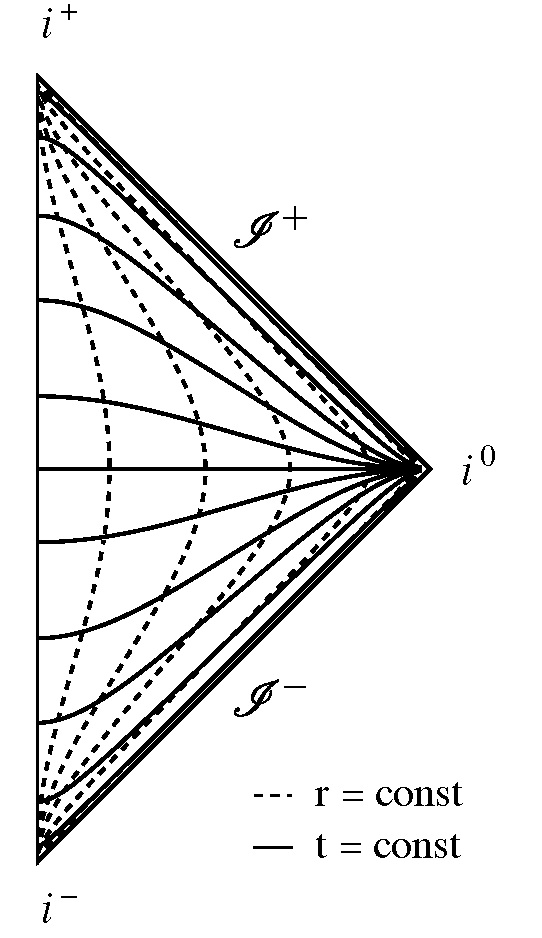
\includegraphics[width =0.3\textwidth]{Penrose diagram.pdf}
    \caption{Penrose Diagram - Representation of the standard
      compactification of the Minkowski spacetime alongside the curves of constant
      time, solid black lines, and the curves of constant r, dotted
      black lines.}
\end{figure}
\\
In this representation we can see that the spatial infinity, $i^0$, is mapped to the origin and $\mathscr{I}^{\pm}$ and to the future/past null cone through the origin.\\

\begin{figure}[h]
	\centering 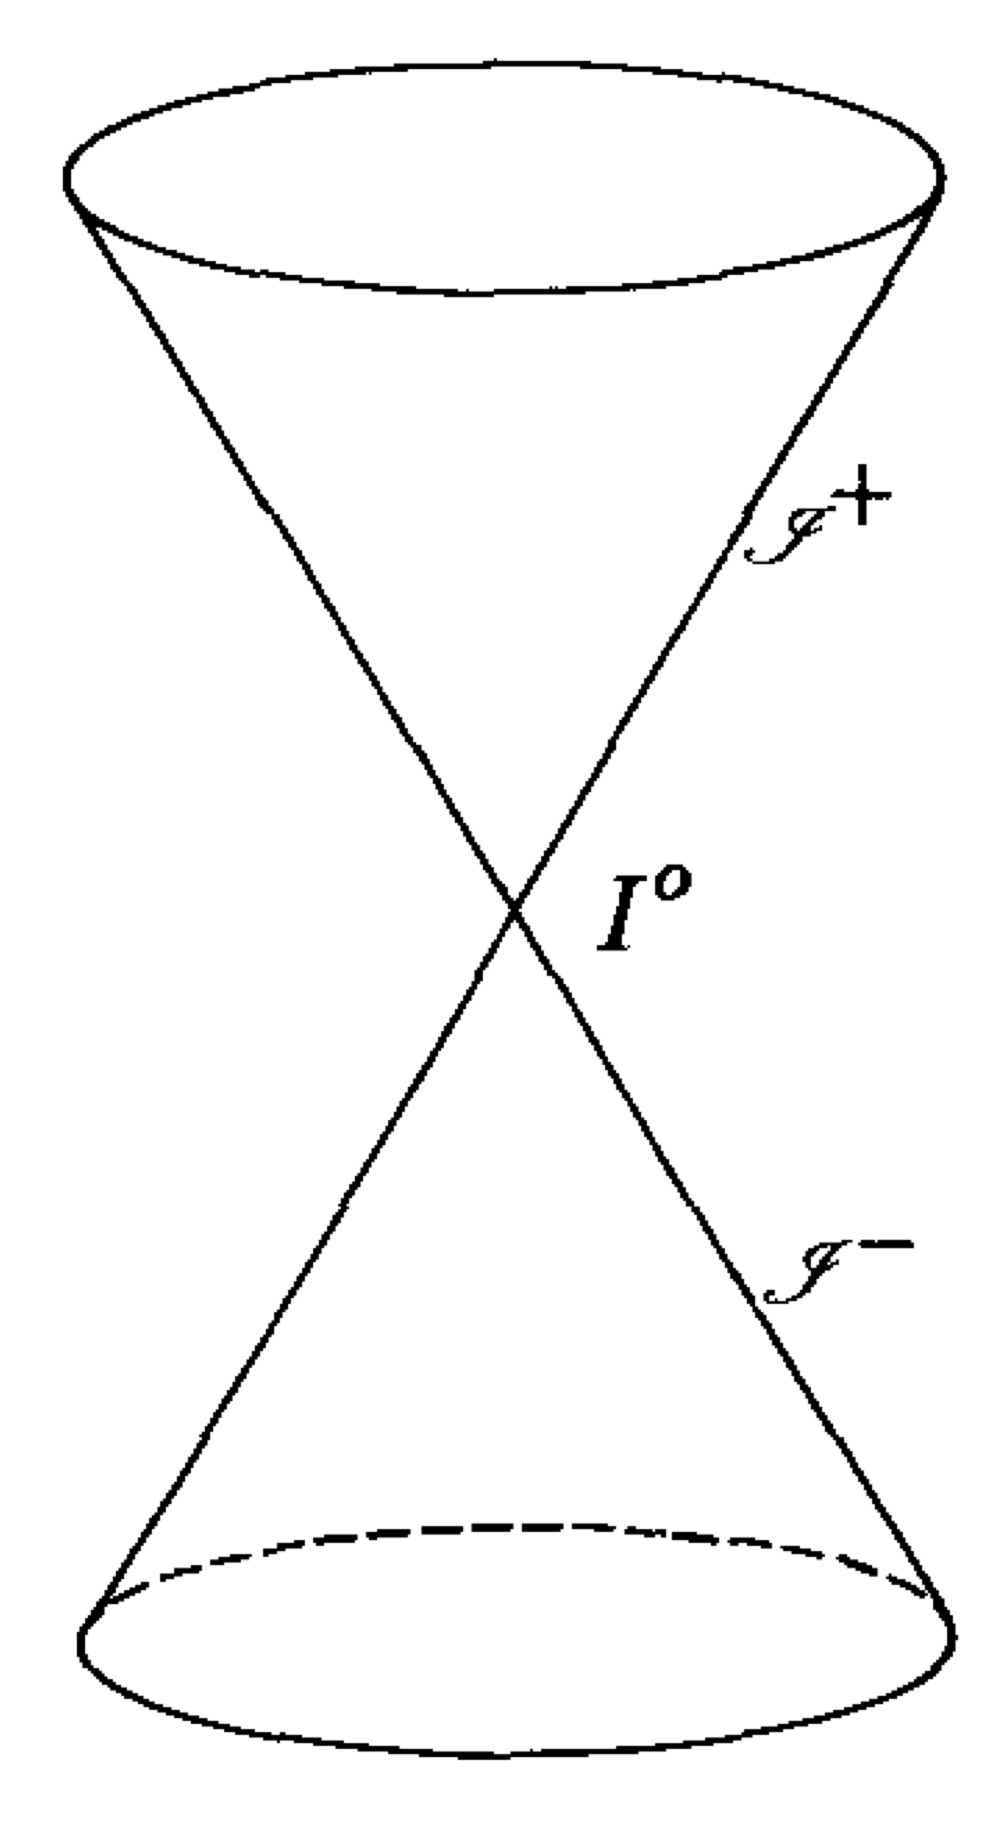
\includegraphics[width =0.3\textwidth]{spatial infinity.jpeg}
    \caption{Representation of spatial infinity, $i^0$, in the Penrose Diagram.\\ Taken from \cite{Ste91}.}
\end{figure}
%%%%%%%%%%%%%%%%%%%%%%%%%%%%%%%%%%%%%%%%%%%%%%%%%%%%%%%%%%%%%%%%%%%%%%%%
\section{Newman-Penrose constants}
\label{section:Newman-Penrose Constants}
The Newman-Penrose constants, originally introduced in \cite{NewPen68}, are quantities defined on null infinity that obey conservation laws for asymptotically flat gravitational fields. For linear fields propagating in flat spacetime, there exists an infinite number of conservation laws. For example, in ordinary Electromagnetic (EM) theory with a spin-1 field, the total charge is conserved. In the linearized gravitational theory, which involves a spin-2 field, the total mass, linear momentum, and angular momentum are also conserved. In our case, we are interested in studying spin-0 fields, which correspond to solutions of the wave equation.\\

The NP constants form an infinite hierarchy of conserved quantities for linear equations, including the spin-1, spin-2, and spin-0 fields. Newman and Penrose demonstrated that these constants can be expressed as the product of the square of the dipole moment and the difference between the monopole and the quadrupole moments, as shown in \cite{DaiVal02}. However, in the full non-linear gravitational theory, the conservation of mass and momentum no longer holds.\\

Turning our attention to the interpretation of these charges, the NP constants are considered a set of conserved charges at null infinity \cite{NewPen68}. These charges are computed as 2-surface integrals at cuts ${C} \approx \mathbb{S}^2$ of null infinity $\mathscr{I}$. In the linear theory, an infinite hierarchy of these conserved quantities exists, while in the non-linear theory of General Relativity, only ten quantities remain conserved \cite{NewPen68}.\\

A conservation law arises when the value of an integral remains constant regardless of the specific "time" at which a 2-surface is selected. In the context of our current investigation, we can determine whether outgoing waves carry away or preserve the quantity of interest by computing the integral at future null infinity with a constant retarded time $u = u_0$, and then comparing it with the integral at a later retarded time $u = u_1$. The difference between the two integrals will capture the contribution from the outgoing waves that escape between the two hypersurfaces defined by $u = \text{constant}$. If this difference always vanishes, then we have a conserved quantity. On the other hand, if the difference does not vanish, then the quantity is not conserved.\\

\begin{figure}[h]
  \centering 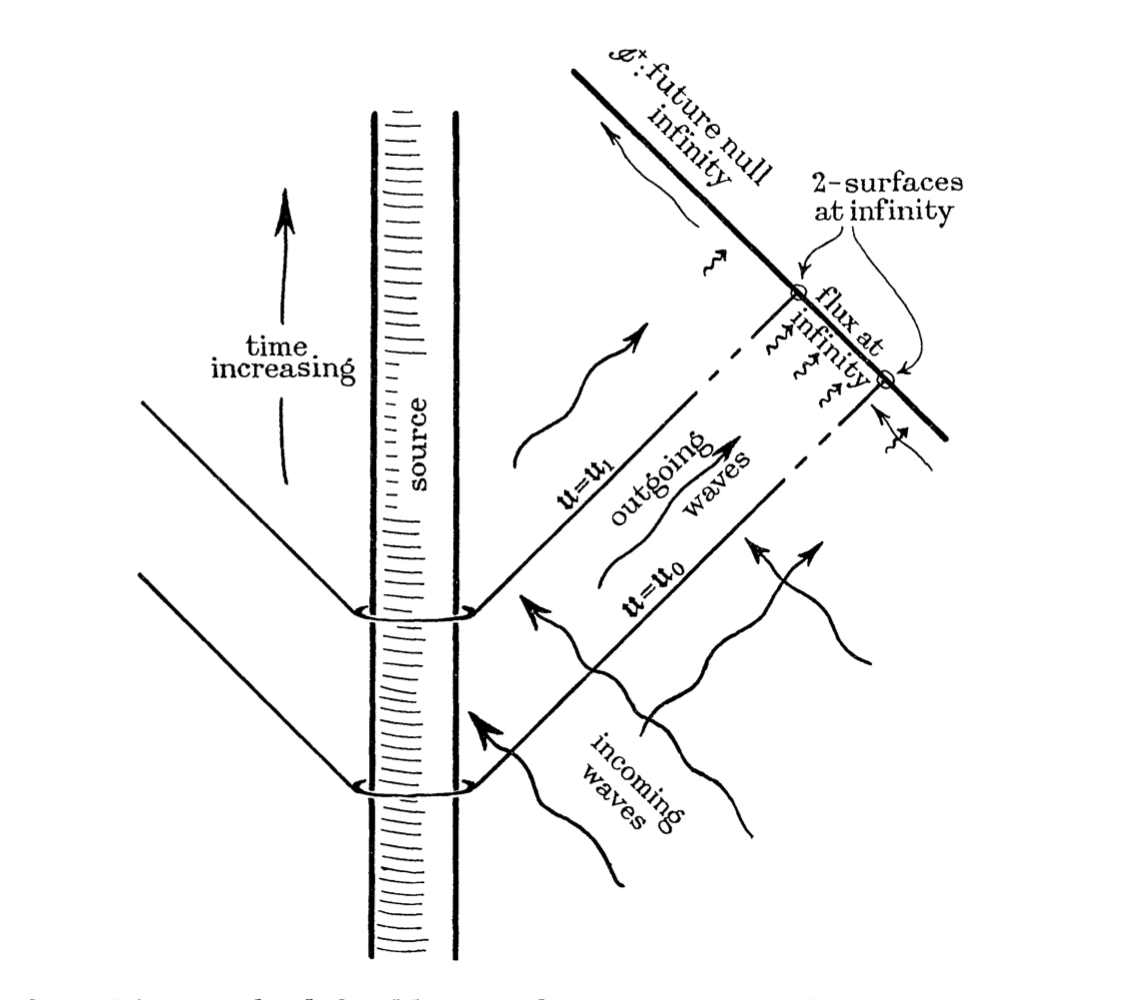
\includegraphics[width =0.55\textwidth]{penrose constants.png}
    \caption{Visual representation of the behavior of the Newman-Penrose constants at null infinity.\\
    Taken from \cite{NewPen68}.}
\end{figure}

The newly (in 1968) discovered conservation laws are distinct and not connected to any previously known laws. While a comprehensive physical interpretation of these new quantities is not yet evident, a preliminary understanding of their significance can be proposed. This interpretation is largely based on their meaning in the linear theories, where their conservation is relatively straightforward, as well as their interpretation in the context of static fields. To gain deeper insights, we will conduct a detailed analysis of the linear gravitational and Maxwell theories. Through this investigation, we hope to shed light on the nature and implications of these novel conservation laws.\\

In the context of flat spacetime, we will introduce a set of null polar coordinates, where the usual spherical polar angles, $\theta$ and $\phi$, are retained. However, we will introduce new coordinates, $r$ and $u$, such that $r/\sqrt{2}$ represents the radial distance, and $(2u - r)/\sqrt{2}$ serves as the time parameter in the standard system. Consequently, $\sqrt{2u}$ corresponds to the conventional retarded time parameter, while $\sqrt{2(u + r)}$ represents the corresponding advanced time. The hypersurfaces defined by $u = \text{constant}$ are the outgoing null cones with their vertices at $r = 0$. The metric is given by:
\begin{equation}\label{eq:flatmetric}
  d s^2 = 2d u^2 + 2dudr - \frac{1}{2} r^2(d\theta^{2} + \sin^2\theta d\phi^2) = g_{\mu \nu}dx^{\mu}dx^{\nu}.
\end{equation}

with 
\begin{equation}
  x^0 = u, \quad x^1 = r, \quad x^2 = \theta, \quad x^3 = \phi.
\end{equation}

At any point in spacetime, a complex tetrad can be selected as follows: The vector $l^{\mu}$ represents the outward null direction tangent to the cone defined by $u = \text{const.}$, while $n^{\mu}$ points inward and is the null vector directed toward $r = 0$. Additionally, $m^{\mu}$ and $\overline{m}^{\mu}$ are complex vectors tangent to the two-dimensional sphere formed by constant $r$ and $u$. In the given null coordinate system, these vectors are chosen to have the form 
\begin{align}\label{eq:tetrad}
  & l^{\mu} = \delta_{1}^{\mu}, \quad n^{\mu} = \delta_{0}^{\mu} - \delta_{1}^{\mu}, \nonumber \\
  & m^{\mu} = \displaystyle\frac{1}{\tau}\left(\delta_{2}^{\mu} + \displaystyle\frac{1}{\sin\theta}\ \delta_{3}^{\mu}\right), \qquad \overline{m}^{\mu} = \displaystyle\frac{1}{\tau}\left(\delta_{2}^{\mu} - \displaystyle\frac{1}{\sin\theta}\ \delta_{3}^{\mu}\right).
\end{align}
To describe the electromagnetic (EM) field, we make use of three complex tetrad components of the Maxwell field tensor denoted as $F_{\mu \nu}$. These components are defined as follows:
\begin{align}\label{eq:Maxtensor}
  & \Phi_{0} = F_{\mu \nu}l^{\mu}n^{\nu}, \nonumber \\
  & \Phi_{1} = \frac{1}{2} F_{\mu \nu}(l^{\mu}n^{\nu} + \overline{m}^{\mu}m^{\nu}), \nonumber \\
  & \Phi_{2} = F_{\mu \nu}\overline{m}^{\mu}n^{\nu}.
\end{align}
Using \eqref{eq:tetrad}, we can express the Maxwell field tensor in terms of the tetrad components as follows:
\begin{align}\label{eq:Maxtensorintetrad}
  & \Phi_{0} = 2^{\frac{-1}{2}}(\boldsymbol{E} + i\boldsymbol{B})\cdot \boldsymbol{m}, \nonumber \\
  & \Phi_{1} = \frac{1}{2}(\boldsymbol{E} + i\boldsymbol{B})\cdot \boldsymbol{c} , \nonumber \\
  & \Phi_{2} = -2^{\frac{-1}{2}}(\boldsymbol{E} + i\boldsymbol{B})\cdot \boldsymbol{\overline{m}}.
\end{align}
From \eqref{eq:Maxtensor} we can see that $\Phi_{0}$, $\Phi_{1}$ and $\Phi_{2}$ have spin weights of 1, 0 and -1, respectively. Thus, we can write the Maxwell equations in terms of $\Phi$, the null polar coordinates and the operator $\dh$ in the following way,
\begin{align}\label{eq:MaxwellEqns}
  & \Biggl(\frac{\partial}{\partial r} + \frac{2}{r}\Biggr)\Phi_{1}  + \frac{1}{r}\dh \Phi_{0} = 0, \\ 
  & \Biggl(\frac{\partial}{\partial r} + \frac{1}{r}\Biggr)\Phi_{2}  + \frac{1}{r}\dh \Phi_{1} = 0, \\ 
  & \Biggl(\frac{\partial}{\partial u} - \frac{\partial}{\partial r} - \frac{1}{r}\Biggr)\Phi_{0}  + \frac{1}{r}\dh \Phi_{1} = 0, \\ 
  & \Biggl(\frac{\partial}{\partial u} - \frac{\partial}{\partial r} - \frac{2}{r}\Biggr)\Phi_{1}  + \frac{1}{r}\dh \Phi_{2} = 0. 
\end{align}
Where $\dh$ is given by $$\dh \eta = -(\sin \theta)^{s}\Biggl(\frac{\partial}{\partial \theta} + \frac{i}{\sin \theta}\frac{\partial}{\partial \phi}\Biggr)\{(\sin \theta)^{-s}\eta\},$$ where $s$ represents the spin weight.
\\
Using this notation, it becomes easy to establish a set of orthogonal functions that achieve completeness on the sphere and also function as eigenfunctions of the operator $\dh \overline{\dh}$. The conventional spherical harmonics are denoted as $Y_{\ell m}(\theta, \phi)$. The spin-weighted spherical harmonics can be defined in the following manner \cite{Ste91}:
\begin{equation}\label{eq:sphericalharmonics}
  { }_0 Y_{l m}(\theta, \phi)=Y_{l m}(\theta, \phi),
\end{equation}
\begin{equation}\label{eq:spinweightSH}
  { }_s Y_{l m}(\theta, \phi)= \begin{cases}(-1)^s R^s\left[2^s \frac{(l-s) !}{(l+s) !}\right]^{1 / 2} \dh^s Y_{l m}(\theta, \phi) & 0 \leq s \leq l \\ R^{-s}\left[2^{-s} \frac{(l+s) !}{(l-s) !}\right]^{1 / 2} \overline{\dh}^{-s} Y_{l m}(\theta, \phi) & 0 \geq s \geq-l \\ 0 & \text { otherwise. }\end{cases}
\end{equation}
\\
Our focus lies on solutions that fulfill a suitable asymptotic boundary condition. This condition allows for all sufficiently smooth retarded fields and includes fields with incoming waves that decay appropriately. We employ the integer $N$ to gauge the degree of smoothness needed, and our requirement is as follows:
\begin{equation}\label{eq:MaxwellAnsatz}
  \phi_{0}=\sum_{n=0}^{N}\frac{\phi_{0}^{n}(u,\theta,\phi)}{r^{3+n}}+o(r^{-3-N}),
\end{equation}
we must assume that the derivatives $r$, $\theta$, $\phi$ and $u$ of \eqref{eq:MaxwellAnsatz} hold. Then, \eqref{eq:MaxwellAnsatz} also controls the behavior of $\Phi_{1}$ and $\Phi_{2}$.\\
Once equations (1.12) and (1.13) are integrated, they yield
\begin{equation}\label{eq:Phi1}
  \Phi_{1} = \frac{\Phi_{1}^{0}}{r^2} + \sum_{n=0}^{N}\frac{\overline{\dh} \phi_{0}^{n}}{(n+1)r^{3+n}}+o(r^{-3-N}),
\end{equation}

\begin{equation}\label{eq:Phi2}
  \Phi_{2} = \frac{\Phi_{2}^{0}}{r} + \frac{1}{r^2}\overline{\dh} \Phi_{1}^{0} + \sum_{n=0}^{N}\frac{\overline{\dh}^2 \phi_{0}^{n}}{(n+1)(n+2)r^{3+n}}+o(r^{-3-N}).
\end{equation}
Substituting into equations (1.14) and (1.15), we obtain the following
\begin{equation}\label{eq:Phi0}
  \dot{\Phi}_{1}^{0} = -\dh\Phi_{2}^{0}, \quad \dot{\Phi}_{0}^{0} = -\dh \Phi_{1}^{0}
\end{equation}
Using  $\overline{\dh}\dh \eta - \dh \overline{\dh} \eta = 2s\eta$, we can write
\begin{equation}\label{eq:Phin+1}
  (n + 1)\dot{\Phi}_{0}^{n+1} = -\{\overline{\dh}\dh \Phi_{0}^{n} + (n+3)n\Phi_{0}^{n}\} \qquad (N \textgreater n \geq 0).
\end{equation}
Before proceeding to derive the new conservation laws, it is essential to first exhibit the law of conservation of charge within this formalism. To achieve this, we multiply the first equation of \eqref{eq:Phi0} by $_{0}Y_{0,0}$ and subsequently integrate over the sphere, yielding:
\begin{equation}\label{eq:YPhi0}
  \frac{d}{du} \int {_{0}Y_{0,0}\Phi_{1}^{0} d\omega} = - \int {_{0}Y_{0,0}\dh \Phi_{2}^{0} d\omega} = 0
\end{equation}
with $\int{_{s}Y_{l,m}\dh^{l-s+1}\xi d\omega} = 0$. Therefore, $\int {_{0}Y_{0,0}\Phi_{1}^{0} d\omega}$ is constant and proportional to the total electric charge.\\
Using the same approach, we can obtain the new conserved quantities multiplying \eqref{eq:Phin+1} by $_{1}\overline{Y}_{n-k+1,m}$ and integrating over the sphere $\int {_{s}\overline{Y}_{l,m}\overline{\dh}\dh \eta d \omega} = -(l-s)(l+s+1) \int{_{s}\overline{Y}_{l,m}\eta d\omega}$:
\begin{equation}\label{eq:Eleccharge}
  (n+1)\frac{d}{du}\int{_{1}Y_{n-k+1,m}\Phi_{0}^{n+1} d\omega} = - \int{_{1}\overline{Y}_{n-k+1,m}(\overline{\dh}\dh \Phi_{0}^{n}+(n+3)n\Phi_{0}^{n})d\omega} = -k(2n-k+3)\int{_{1}\overline{Y}_{n-k+1,m}\Phi_{0}^{n} d\omega}.
\end{equation}
Consequently,
\begin{equation}\label{eq:F}
  F_{m}^{n,k} = \int{_{1}\overline{Y}_{n-k+1,m}\Phi_{0}^{n+1} d\omega},
\end{equation}
where $m$, $n$ and $k$ satisfy $n \geq k \geq 0$, $|m| \leq n-k+1$, and therefore 
\begin{equation}\label{eq:Fdot}
  \dot{F}_{m}^{n,k} = \frac{-k(2n-k+3)}{(n+1)}F_{m}^{n-1,k-1} ; \qquad \dot{F}_{m}^{n,0} = 0.
\end{equation}
As a result, we obtain a series of conserved quantities denoted as $F_{m}^{n,0}$ (when $N \geq n+1$). Nevertheless, in the non-linear Einstein-Maxwell theory, only certain quantities for $n = 0$ and $m = -1, 0, 1$ remain conserved. Hence, our main focus will be on these three quantities, and we will use the shorthand notation $F_{m} = F_{m}^{0,0}$.\\
From the following ansatz
\begin{equation}\label{eq:Phi0ansatz}
  \Phi_{0}^{n} = \sum_{l = n+1}^{\infty}\alpha_{l,m}^{n} {_{1}Y_{l,m}},
\end{equation}
for all outgoing multipole solutions (with sufficient smoothness), the coefficients $F_{m}^{n,k}$ are zero in the absence of incoming waves. These coefficients, $F_{m}^{n,k}$, provide a measure of the asymptotic properties of the time profile of the incoming waves for large values of the advanced time coordinate $v = u + r$. In this analysis, we will particularly focus on the case of an incoming dipole field with the dipole axis along the z-direction.\\
The field of the advanced dipole described with retarded coordinates is as follows:
\begin{align}\label{eq:RetardCoordsPhi}
  & \phi_{0} = -\sin\theta \frac{\partial^{2}}{\partial r^{2}}\left(\frac{\alpha}{r}\right), \nonumber \\ 
  & \phi_{1} = -2 \cos\theta \frac{\partial}{\partial r}\left(\frac{\alpha}{r^2}\right), \nonumber \\ 
  & \phi_{2} = +2 \sin\theta \frac{\alpha}{r^{3}},
\end{align}
in the above expression, $\alpha = \alpha(u + r)$ is an arbitrary complex function of the advanced time $u + r$ and represents the electric dipole moment plus $i$ times the magnetic dipole moment.
To verify the validity of this solution, we can perform a direct substitution of the given expression in the Maxwell equations (1.12)-(1.15). To satisfy the condition \eqref{eq:MaxwellAnsatz}, we must assume (taking $N = 1$):
$$\alpha = \beta(u+r)^{-1} + o((u+r)^{-1})$$
Plugging into \eqref{eq:RetardCoordsPhi} and making use of the following identity $(u+r)^{-1} = r^{-1}-ur^{-2}+u^{2}r^{-3}$, we obtain:
\begin{equation}\label{eq:Phi0retard}
  \Phi_{0} = -6\beta r^{-4}\sin\theta + o(r^{-4}),
\end{equation}
and with \eqref{eq:MaxwellAnsatz}, $\Phi_{0}^{1} = -6\beta \sin\theta$ and \eqref{eq:F}, $$F_{0} = -8(3\pi)^{-\frac{1}{2}}\beta, \qquad F_{-1} = F_{1} = 0.$$
Hence, the $F_m$ values are determined solely by the coefficient of the $(u + r)^{-1}$ term in the asymptotic expansion of the incoming dipole field. Consequently, in flat spacetime, they may not carry significant fundamental significance. A similar observation applies to the other $F_{m}^{n,k}$ quantities.\\

Furthermore, these conclusions and results obtained in the context of Maxwell theory can be straightforwardly extended to the case of linearized gravitational theory. The five complex functions:
\begin{align}\label{eq:MaxcomplexFuc}
  & \Psi_{0} = -C_{\mu\nu\rho\sigma}l^{\mu}m^{\nu}l^{\rho}m^{\sigma}, \nonumber \\ 
  & \Psi{1} = -C_{\mu\nu\rho\sigma}l^{\mu}n^{\nu}l^{\rho}m^{\sigma}, \nonumber \\ 
  & \Psi_{2} = -C_{\mu\nu\rho\sigma}{\overline{{{m}}}^{\mu}n^{\nu}l^{\rho}m^{\sigma}}, \nonumber \\ 
  & \Psi_{3} = -C_{\mu\nu\rho\sigma}{\overline{{{m}}}^{\mu}n^{\nu}l^{\sigma}}n^{\sigma}, \nonumber \\
  & \Psi_{4} = -C_{\mu\nu\rho\sigma}{\overline{{{m}}}^{\mu}n^{\nu}\overline{{{m}}}^{\rho}}n^{\sigma}
\end{align}
In the context of linearized gravitational theory, we introduce the five complex functions denoted by $\Psi$, where $C_{\mu\nu\rho\sigma}$ represents the linearized Weyl tensor. These functions play an analogous role to the $\Phi$'s in the Maxwell theory. Their dynamics are governed by the linearized Bianchi identities. Much like the correspondence between $F_{\mu \nu}$ and the electromagnetic fields $(\boldsymbol{E}, \boldsymbol{B})$, the linearized Weyl tensor corresponds to two trace-free symmetric, 3-dimensional tensors denoted as $C_{km}$ and $E_{km}$, with $C_{km}$ given by $C_{\alpha \kappa \beta \mu}(l^{\alpha}+n^{\alpha})(l^{\beta}+n^{\beta})$ and $E_{km}$ given by $C_{\alpha \kappa \beta \mu}^{*}(l^{\alpha}+n^{\alpha})(l^{\beta}+n^{\beta})$. Writting $$Z_{k,j} = \frac{1}{2}C_{k,j} + \frac{i}{2}E_{k,j},$$ we get $$\Psi_{0} = - Z_{k,j}m_{k}m_{j}, \qquad \Psi_{1} = 2^{\frac{1}{2}}Z_{k,j}c_{k}m_{j}, \qquad \Psi_{2} = Z_{k,j}m_{k}\overline{m}_{j}, \qquad \Psi_{3} = - 2^{\frac{1}{2}}Z_{k,j}c_{k}\overline{m}_{j}, \qquad \Psi_{4} = -Z_{k,j}\overline{m}_{k}\overline{m}_{j}.$$

Similar to the Maxwell theory, our focus lies on solutions that satisfy a boundary condition at infinity, allowing for sufficiently smooth retarded fields and properly tailing off incoming fields. Specifically, we demand behavior of the form:
\begin{equation}\label{eq:Psi0ansatz}
  \Psi_{0}=\sum_{n=0}^{N}\frac{\Psi_{0}^{n}}{r^{5+n}}+(o^{-5-N}),
\end{equation}
under these conditions, the 'Bianchi identities' can be integrated to yield:
\begin{align}\label{eq:Psiintegrals}
  & \Psi_{1}=\frac{\Psi_{1}^{0}}{r^{4}}+o({r}^{-4}), \nonumber \\ 
  & \Psi_{2}=\frac{\Psi_{2}^{0}}{r^{3}}+o({r}^{-3}), \nonumber \\ 
  & \Psi_{3}=\frac{\Psi_{3}^{0}}{r^{2}}+o({r}^{-2}), \nonumber \\
  & \Psi_{4}=\frac{\Psi_{4}^{0}}{r}+o({r}^{-1}).
\end{align}

After employing equations \eqref{eq:Psi0ansatz}, \eqref{eq:Psiintegrals}, and $\dh$, the time-development equations (the second set of the Bianchi identities) take the following form:
\begin{equation}\label{eq:Psidot}
  \dot{\Psi}_{0}^{0} = -\dh \Psi_{1}^{0}, \qquad \dot{\Psi}_{1}^{0} = -\dh \Psi_{2}^{0}, \qquad \dot{\Psi}_{2}^{0} = -\dh \Psi_{3}^{0}, \qquad \dot{\Psi}_{3}^{0} = -\dh \Psi_{4}^{0}.
\end{equation}

\begin{equation}\label{eq:Psi0n+1}
  (n+1)\dot{\Psi}_{0}^{n+1} = -\{\overline{\dh}\dh + (n+5)n\}\Psi_{0}^{n} \qquad (N \textgreater n \geq 0).
\end{equation}

The conservation of mass can be derived using equation \eqref{eq:Psidot} in a manner analogous to how the conservation of charge was obtained from equation \eqref{eq:Phi0}
\begin{equation}\label{eq:YPsi0}
  \frac{d}{du} \int {_{0}Y_{0,0}\Psi_{2}^{0} d\omega} = - \int {_{0}Y_{0,0}\dh \Psi_{3}^{0} d\omega} = 0.
\end{equation}
The total mass is proportional to the function $\int {_{0}Y_{0,0}\Psi_{2}^{0} d\omega}$. Demonstrating the conservation laws for linear and angular momentum requires a more involved approach, as their proofs rely on the existence of the linearized metric tensor and the Weyl tensor. The crucial significance of the existence of the linearized metric lies in implying that the dipole parts of $\Psi_{3}^{0}$ and $\Psi_{2}^{0}$ are purely 'magnetic' and 'electric', respectively. The linear momentum vector is given by
\begin{equation}\label{eq:LinMomentum}
  \int {_{0}Y_{1,m}Re(\Psi_{2}^{0}) d\omega} = \Biggl(\int{_{0}Y_{1,m}\Psi_{2}^{0} d\omega} \Biggr)
\end{equation}
and the angular momentum vector
\begin{equation}\label{eq:AngMomentum}
  \int {_{0}Y_{1,m}Im(\overline{\dh} \Psi_{1}^{0}) d\omega} \quad (m = -1,0,1).
\end{equation}

In the linear theory, the new conservation laws can be derived from equation \eqref{eq:Psi0n+1} by multiplying both sides by $_{2}\overline{Y}_{n-k+2,m}$ and integrating over the sphere:
\begin{equation}\label{eq:intYoverline}
  (n+1)\frac{d}{du}\int{_{2}\overline{Y}_{n-k+2,m}\Psi_{0}^{n+1} d\omega} = - \int{_{2}\overline{Y}_{n-k+2,m}\{\overline{\dh}\dh \Psi_{0}^{n}+(n+5)n\Psi_{0}^{n}\}d\omega} = -\int{_{2}\overline{Y}_{n-k+2,m}k(2n-k+5)\Psi_{0}^{n} d\omega},
\end{equation}
hence 
\begin{equation}\label{eq:Gdot}
  \dot{G}_{m}^{n,k} = \frac{-k(2n-k+5)}{(n+1)}G_{m}^{n-1,k-1} ; \qquad \dot{G}_{m}^{n,0} = 0.
\end{equation}
where $m$, $n$ and $k$ satisfy $n \geq k \geq 0$, $|m| \leq n-k+2$, with
\begin{equation}\label{eq:G}
  G_{m}^{n,k} = \int{_{1}\overline{Y}_{n-k+2,m}\Phi_{0}^{n+1} d\omega}.
\end{equation}

The interpretation of these charges is still a subject of debate [\cite{PenRin84}, \cite{DaiVal02}, \cite{Bac10}]. However, their conservation holds in
general asymptotically flat spacetimes, even when the dynamics involve complex phenomena like black hole
collisions \cite{DaiVal02}. Recent interest in asymptotic quantities, particularly the Bondi-Metzner-Sachs (BMS) charges,
has emerged due to their connection with the concept of black hole soft hair [\cite{HawMalStr16}, \cite{HawMalStr17}, \cite{HeLyMi15}]. Understanding the relationship between conserved quantities at past and future null infinity is a crucial aspect of these discussions.\\

However, the resolution of the singular nature of spatial infinity poses challenges in matching the conserved
quantities.
Therefore, the study of the Newman-Penrose constants and their conservation offers valuable insights into the
dynamics of gravitational fields, particularly in black hole collisions and asymptotically flat spacetimes. These
constants provide information about the residual radiation and behavior of the system at later times, shedding
light on the intricate nature of spacetime and the conservation laws that govern it.\\

%%%%%%%%%%%%%%%%%%%%%%%%%%%%%%%%%%%%%%%%%%%%%%%%%%%%%%%%%%%%%%%%%%%%%%%%%%%%%%%%%%%%%%%%%%%%%%%%%%%%%%%%%%%%%%%%%%%
\section{Peeling Theorem}
\label{sec:Peeling Theorem}

The peeling theorem, one of the most emblematic results in the classical theory of asymptotics in general relativity, has played a very important role in the development of the modern notion of gravitational radiation. It
is usually formulated within the context of asymptotically simple spacetimes, as defined in Section 10.2 of \cite{Val16}.
An inspection of the proof of the peeling theorem reveals that, in fact, it is only necessary to assume that the
conformal extension is $\mathbb{C}^4$. In view of this, the question of the existence and genericity of spacetimes satisfying the peeling behavior can be rephrased in terms of the construction of asymptotically flat spacetimes with, at least, this minimum of differentiability \cite{GasVal17}. Penrose’s compactification procedure, when applied to the
Minkowski spacetime, yields a fully smooth conformal extension. However, for spacetimes with nonvanishing
mass, such as the Schwarzschild spacetime, the conformal structure degenerates at spatial infinity. This degen-
eration occurs because spatial infinity can be viewed as the final point of the generators of null infinity, either
in the past or future direction. As a result, it is natural to expect that the behavior of the gravitational fields near
spatial infinity will somehow reflect the peeling properties of the spacetime \cite{Pen65a}.\\

In the context of the physical Ricci tensor vanishing near infinity, the physical Weyl tensor $C_{abcd}$ contains all essential information about the curvature in the region. Being conformally invariant, it is related to the unphysical Weyl tensor $\tilde{C}_{abcd}$ as $C_{abcd} = \tilde{C}_{abcd}$. The critical point to note is that $\tilde{C}_{abcd}$ must vanish at $\mathscr{I}^+$. \\

Now, consider any null geodesic $\gamma$ within spacetime $M$ from a point $p$ in the physical region to another point $q$ on $\mathscr{I}^+$. Let $\lambda$ be the physical affine parameter along $\gamma$, where $q$ corresponds to the limit as $\lambda$ tends to infinity. The tangent vector $k^{a}$ to $\gamma$ in this parameterization plays a vital role. While the unphysical Weyl curvature on $\gamma$ may not have any specific characteristics, it is guaranteed to vanish at $q$. However, during the transformation from unphysical to physical spacetime, an infinite amount of "stretching" occurs along the direction of $k^{a}$. This results in the peeling property of the physical Weyl tensor, which can be expressed as follows: As $\lambda$ approaches infinity, we observe that:
\begin{equation}\label{eq:peeling}
  C_{a b c d}=\frac{C_{a b c d}^{(1)}}{\lambda}+\frac{C_{a b c d}^{(2)}}{\lambda^{2}}+\frac{C_{a b c d}^{(3)}}{\lambda^{3}}+\frac{C_{a b c d}^{(4)}}{\lambda^{4}}+O\Bigl(\frac{1}{\lambda^{5}}\Bigr),
\end{equation}
in the context of an asymptotically Minkowski spacetime basis, each component of the physical Weyl tensor, denoted as $C_{abcd}^{\mu}$, exhibits bounded behavior \cite{Wal84a}. \\

The peeling theorem, documented in [\cite{Sac61}, \cite{BonBurMet62}, \cite{NewPen62}], represents a significant outcome in the study of asymptotic behavior in general relativity. It characterizes the decay of the Weyl tensor in the asymptotic region of
the spacetime, signifying the gradual "peeling" of gravitational radiation. This theorem deepens our understanding of the intricate nature of gravitational radiation and its properties in the far reaching regions of the spacetime.\\

Hence, the peeling theorem and the Newman-Penrose constants are interconnected concepts that deepen our
understanding of the gravitational radiation and its properties in asymptotically flat spacetimes.
%%%%%%%%%%%%%%%%%%%%%%%%%%%%%%%%%%%%%%%%%%%%%%%%%%%%%%%%%%%%%%%%%%%%%%%%%%%%%%%%%%%%%%%%%%%%%%%%%%%%%%%%%%%%%%%%%%%%%%
\section{The Newman-Penrose gauge}
\label{sec:The Newman-Penrose gauge}

The Peeling theorem underscores the advantages of adopting a gauge that is well-suited to the structure of null infinity. By utilizing the Newman-Penrose gauge, we gain even deeper insights into the properties of asymptotically simple spacetimes. This gauge choice allows for a more comprehensive understanding of the behavior and characteristics of these spacetimes at infinity \cite{Val16}. \\

Let us consider a conformal extension $(M, \boldsymbol{g}, \Xi)$ of an asymptotically simple spacetime $(\tilde{M}, \tilde{\boldsymbol{g}})$, where $\tilde{\boldsymbol{g}}$ satisfies the vacuum Einstein field equations with a cosmological constant of zero. In the theory of asymptotics, it is known that for vacuum spacetimes with zero cosmological constant, the conformal boundary $\mathscr{I}$ is composed of two distinct null hypersurfaces: $\mathscr{I}^+$ and $\mathscr{I}^-$. Both hypersurfaces have the topological structure of $\mathbb{R} \times  \mathbb{S}^2$.\\

In the forthcoming exposition, we shall use the symbol $\{l^{\prime}, n^{\prime}, m^{\prime}, \overline{m}^{\prime}\}$ to denote a frame defined in a local region $U$ around $\mathscr{I}^+$. This frame will be referred to as "adapted to $\mathscr{I}^+$ " provided it satisfies the following conditions:

\begin{itemize}
  \item[(i)] The vector $l^{\prime}$ is tangential to $\mathscr{I}^{+}$ and remains parallelly propagated along this null hypersurface, which can be expressed as follows:
   \begin{equation*}
   \nabla_{l^{\prime}} l^{\prime} \simeq 0.
   \end{equation*}
  \item[(ii)] Within $U$, we can find a smooth function $u$ that acts as an affine parameter along the null generators of $\mathscr{I}^{+}$, denoted by $l^{\prime}(u) \simeq 1$. We then define the vector $n^{\prime}$ as $n^{\prime}=\boldsymbol{g}(\mbox{\textbf{d}}u, \cdot )$, which makes it tangential to the null generators of the hypersurfaces transverse to $\mathscr{I}$ defined by:
  \begin{equation*}
  \mathcal{N}_{u_{\circ}}\equiv \{ p \in U \;| \; u(p)=u_{\circ}\},
  \end{equation*}
   with constant $u_{\circ}$.
  \item[(iii)] The tetrad $\{l^{\prime}, n^{\prime}, m^{\prime}, \overline{m}^{\prime}\}$ is aligned with the tangent vectors of the cuts $\mathcal{C}_{u_{\circ}}\equiv \mathcal{N}_{u_{\circ}}\cap \mathscr{I}^{+} \approx \mathbb{S}^2$, and it is parallelly propagated along $\mathcal{N}_{u_{\circ}}$, meaning that it fulfills the condition:
  \begin{equation*}
  \nabla_{n^{\prime}}\{l^{\prime}, n^{\prime}, m^{\prime}, \overline{m}^{\prime}\}=0 \qquad \text{on} \qquad
  \mathcal{N}_{u_{\circ}}.
  \end{equation*}
  \end{itemize}


  


















%%%%%%%%%%%%%%%%%%%%%%%%%%%%%%%%%%%%%%%%%%%%%%%%%%%%%%%%%%%%%%%%%%%%%%%%

\chapter{Cylinder at $i^0$}
\label{chapter:cylinder}

In Penrose's conformal approach \cite{Pen63}, the investigation of the gravitational field's decay and the asymptotic structure of spacetime is conducted not with respect to the physical spacetime $(\tilde{\mathcal{M}}, \tilde{\boldsymbol{g}})$ that satisfies the Einstein field equations $\tilde{R}_{a b}=0$. Instead, it is examined in terms of conformally related spacetime $(\mathcal{M}, \boldsymbol{g})$, referred to as the unphysical spacetime, where $\boldsymbol{g}=\Omega^2 \tilde{\boldsymbol{g}}$. The conformal factor $\Omega$ plays a crucial role as a boundary defining function. Specifically, it defines the set of points $\mathscr{I}$ in the unphysical manifold where $\Omega = 0$ while ensuring that $d\Omega \neq 0$. \\

Within the conformal structure of asymptotically flat spacetimes, a distinguished point is spatial infinity $i^0$, characterized by $\Omega = 0$ and $d\Omega = 0$. Extensive discussions on the conformal approach and the conformal Einstein field equations can be found in [\cite{Val16}, \cite{Fra04}, \cite{Fri02}]. This comprehensive exploration delves into the nuances of the conformal methodology and its implications for understanding the asymptotic behavior and structure of spacetime.
%%%%%%%%%%%%%%%%%%%%%%%%%%%%%%%%%%%%%%%%%%%%%%%%%%%%%%%%%%%%%%%%%%%%%%%%

\section{The $i^0$ cylinder representation in Minkowski  spacetime}
\label{the $i^0$ cylinder}

Consider the spherical polar coordinates denoted by $(\tilde{t}, \tilde{\rho}, \vartheta^A)$ with $A = 1, 2$, where $\vartheta^A$ represents a set of coordinates on $\mathbb{S}^2$. In this coordinate system, the metric of \textit{physical} Minkowski spacetime is given by $\tilde{\eta}$
\begin{equation}\label{eq:physicalMikmetric}
\tilde{\boldsymbol{\eta}}=-\mathbf{d} \tilde{t} \otimes \mathbf{d} \tilde{t}+\mathbf{d} \tilde{\rho} \otimes \mathbf{d} \tilde{\rho}+\tilde{\rho}^2 \boldsymbol{\sigma}.
\end{equation}
In the specific range, $\tilde{t} \in (-\infty, \infty)$, $\tilde{\rho} \in [0, \infty)$, where $\sigma$ denotes the standard metric on $\mathbb{S}^2$, we introduce \textit{unphysical} spherical polar coordinates $(t, \rho, \vartheta^A)$ as an intermediate step towards obtaining the desired conformal representation
\begin{equation}\label{eq:unphysicalCoords}
t=\frac{\tilde{t}}{\tilde{\rho}^2-\tilde{t}^2}, \quad \rho=\frac{\tilde{\rho}}{\tilde{\rho}^2-\tilde{t}^2}.
\end{equation}
By expressing the physical Minkowski metric $\tilde{\eta}$ in terms of the unphysical spherical polar coordinates $(t, \rho, \vartheta^A)$, one can easily recognize the \textit{inversion} conformal representation of the Minkowski spacetime $(\mathbb{R}^4, \eta)$, where:
\begin{equation}\label{eq:metricRelation}
  \boldsymbol{\eta} = \Xi^2 \boldsymbol{\tilde{\eta}}.
\end{equation}
Substituting $t$ and $\rho$ into $\Xi$ yields,
\begin{equation}\label{eq:Xi}
  \Xi= \rho^2 - t^2 = \left(\frac{\tilde{\rho}}{\tilde{\rho}^2-\tilde{t}^2}\right)^2 - \left(\frac{\tilde{t}}{\tilde{\rho}^2-\tilde{t}^2}\right)^2 = \frac{\tilde{\rho}^2 - \tilde{t}^2}{(\tilde{\rho}^2-\tilde{t}^2)^2} = \frac{1}{\tilde{\rho}^2 - \tilde{t}^2},
\end{equation}
substituting $\Xi$ into \eqref{eq:metricRelation} yields:
\begin{equation}\label{eq:Unphysicalspacetimemetric}
  \boldsymbol{\eta} = \left(\frac{1}{\tilde{\rho}^2 - \tilde{t}^2}\right)^2 (-\mathbf{d} \tilde{t} \otimes \mathbf{d} \tilde{t}+\mathbf{d} \tilde{\rho} \otimes \mathbf{d} \tilde{\rho}+\tilde{\rho}^2 \boldsymbol{\sigma}) = \frac{1}{(\tilde{\rho}^2 - \tilde{t}^2)^2} (-\mathbf{d} \tilde{t} \otimes \mathbf{d} \tilde{t}+\mathbf{d} \tilde{\rho} \otimes \mathbf{d} \tilde{\rho}+\tilde{\rho}^2 \boldsymbol{\sigma})
\end{equation}
with
\begin{equation}\label{eq:Unphysicalspacetimemetric1}
  \boldsymbol{\eta}=-\mathbf{d} t \otimes \mathbf{d} t+\mathbf{d} \rho \otimes \mathbf{d} \rho+\rho^2 \boldsymbol{\sigma},
\end{equation}
plugging \eqref{eq:Unphysicalspacetimemetric1} into \eqref{eq:Unphysicalspacetimemetric} yields:
\begin{align}\label{eq:Unphysicalspacetimemetric2}
  & \boldsymbol{\eta} = -\mathbf{d} \left(\frac{\tilde{t}}{\tilde{\rho}^2-\tilde{t}^2}\right) \otimes \mathbf{d} \left(\frac{\tilde{t}}{\tilde{\rho}^2-\tilde{t}^2}\right) + \mathbf{d} \left(\frac{\tilde{\rho}}{\tilde{\rho}^2-\tilde{t}^2}\right) \otimes \mathbf{d} \left(\frac{\tilde{\rho}}{\tilde{\rho}^2-\tilde{t}^2}\right) + \left(\frac{\tilde{\rho}}{\tilde{\rho}^2-\tilde{t}^2}\right)^2 \boldsymbol{\sigma} \nonumber \\
  & = -\frac{\mathbf{d} \tilde{t} \otimes \mathbf{d} \tilde{t}}{(\tilde{\rho}^2-\tilde{t}^2)^2}+\frac{\mathbf{d} \tilde{\rho} \otimes \mathbf{d} \tilde{\rho}}{(\tilde{\rho}^2-\tilde{t}^2)^2}+\frac{\tilde{\rho}^2}{(\tilde{\rho}^2-\tilde{t}^2)^2} \boldsymbol{\sigma} \nonumber \\
  & = -\frac{1}{\tilde{\rho}^2-\tilde{t}^2} (\mathbf{d} \tilde{t} \otimes \mathbf{d} \tilde{t}-\mathbf{d} \tilde{\rho} \otimes \mathbf{d} \tilde{\rho}+\tilde{\rho}^2 \boldsymbol{\sigma}).
\end{align}
By comparing the result with the expression \eqref{eq:metricRelation}, we see that they are equal:
\begin{equation}\label{eq:UnphysicalMetricFinal}
  \boldsymbol{\eta} = -\frac{1}{\tilde{\rho}^2-\tilde{t}^2} (\mathbf{d} \tilde{t} \otimes \mathbf{d} \tilde{t}-\mathbf{d} \tilde{\rho} \otimes \mathbf{d} \tilde{\rho}+\tilde{\rho}^2 \boldsymbol{\sigma}) = \boldsymbol{\tilde{\eta}}.
\end{equation}
Hence, the equation \eqref{eq:metricRelation} is equivalent to the given expression for \(\boldsymbol{\eta}\) with the provided expressions for \(t\) and \(\rho\).
In this conformal representation, where $t \in (-\infty, \infty)$, $\rho \in [0, \infty)$, the spatial infinity and the origin undergo an interchange. This implies that $i^0$ is represented by the point $(t = 0, \rho = 0)$ in $(\mathbb{R}^4, \eta)$. Introducing the coordinates $(\tau, \rho, \vartheta^A)$, where $t = \rho \tau$, and considering the conformal metric $\boldsymbol{g} = \rho^{-2} \boldsymbol{\eta}$, we obtain:
\begin{align}\label{eq:unphysicalmetricMink}
  & \boldsymbol{g} = \rho^{-2} \boldsymbol{\eta} = \rho^{-2}(-\rho^{2}\mathbf{d} \tau \otimes \mathbf{d} \tau + \mathbf{d} \rho \otimes \mathbf{d} \rho + \rho^2 \boldsymbol{\sigma}) \equiv \nonumber \\
  & \boldsymbol{g} = -\mathbf{d} \tau \otimes \mathbf{d} \tau + \frac{1}{\rho^2} \mathbf{d} \rho \otimes \mathbf{d} \rho + \boldsymbol{\sigma}.
\end{align}
Expressing $\frac{1}{\rho^2} \mathbf{d} \rho \otimes \mathbf{d} \rho$ in terms of $\tau$ and $\rho$:
\begin{equation}\label{eq:drhotimesdrho}
  \frac{1}{\rho^2} \mathbf{d} \rho \otimes \mathbf{d} \rho = \frac{\left(1-\tau^2\right)}{\rho^2} \mathbf{d} \rho \otimes \mathbf{d} \rho .
\end{equation}
Combining terms with $\frac{1}{\rho^2} \mathbf{d} \rho \otimes \mathbf{d} \rho$ and $\frac{\tau}{\rho} \mathbf{d} \rho \otimes \mathbf{d} \tau$:
\begin{equation}\label{eq:drhotimesdtau}
  \frac{1}{\rho^2} \mathbf{d} \rho \otimes \mathbf{d} \rho + \frac{\tau}{\rho} \mathbf{d} \rho \otimes \mathbf{d} \tau = \frac{1}{\rho^2} \left(1 - \tau^2 - \tau\right) \mathbf{d} \rho \otimes \mathbf{d} \rho .
\end{equation}
Expressing $\frac{\tau}{\rho} \mathbf{d} \tau \otimes \mathbf{d} \rho$ in terms of $\rho$ and $\tau$:
\begin{equation}\label{eq:dtautimesdrho}
  \frac{\tau}{\rho} \mathbf{d} \tau \otimes \mathbf{d} \rho = -\frac{\tau}{\rho} \mathbf{d} \rho \otimes \mathbf{d} \tau .
\end{equation}
Combine the expressions obtained in \eqref{eq:drhotimesdtau} and \eqref{eq:dtautimesdrho} yelds:
\begin{equation}\label{eq:drhotimesdrho1}
  \frac{1}{\rho^2} \left(1 - \tau^2 - \tau\right) \mathbf{d} \rho \otimes \mathbf{d} \rho -\frac{\tau}{\rho} \mathbf{d} \rho \otimes \mathbf{d} \tau = -\frac{\tau}{\rho} \left(\mathbf{d} \rho \otimes \mathbf{d} \tau + \mathbf{d} \tau \otimes \mathbf{d} \rho\right).
\end{equation}
Substitute the expressions obtained in \eqref{eq:drhotimesdrho} and \eqref{eq:drhotimesdrho1} into \eqref{eq:unphysicalmetricMink} gives,
\begin{align}\label{eq:unphysicalmetricMinkFinal}
  & \boldsymbol{g} = -\mathbf{d} \tau \otimes \mathbf{d} \tau + \frac{1}{\rho^2} \left(1 - \tau^2 - \tau\right) \mathbf{d} \rho \otimes \mathbf{d} \rho -\frac{\tau}{\rho} \left(\mathbf{d} \rho \otimes \mathbf{d} \tau + \mathbf{d} \tau \otimes \mathbf{d} \rho\right) + \boldsymbol{\sigma} \nonumber \\
  & = -\mathbf{d} \tau \otimes \mathbf{d} \tau + \frac{1 - \tau^2}{\rho^2} \mathbf{d} \rho \otimes \mathbf{d} \rho -\frac{\tau}{\rho} \left(\mathbf{d} \rho \otimes \mathbf{d} \tau + \mathbf{d} \rho \otimes \mathbf{d} \tau\right) + \boldsymbol{\sigma} \equiv \nonumber \\
  & \boldsymbol{g}=-\mathbf{d} \tau \otimes \mathbf{d} \tau+\frac{\left(1-\tau^2\right)}{\rho^2} \mathbf{d} \rho \otimes \mathbf{d} \rho-\frac{\tau}{\rho} \mathbf{d} \rho \otimes \mathbf{d} \tau-\frac{\tau}{\rho} \mathbf{d} \tau \otimes \mathbf{d} \rho+\boldsymbol{\sigma}.
\end{align}
In this context the \textit{unphyical metric $\boldsymbol{g}$} is related to the physical metric through the following relationship:
\begin{equation}\label{eq:gandtheta}
\boldsymbol{g}=\Theta^2 \tilde{\boldsymbol{\eta}}, \quad \text { where } \quad \Theta:=\frac{\Xi}{\rho}=\rho\left(1-\tau^2\right).
\end{equation}
The unphysical metric $\boldsymbol{g}$, also known as the $i^0$ - cylinder metric, is associated with the coordinates $(\tau, \rho, \vartheta^A)$, which are commonly referred to as the $F$ - coordinates system.
The F-coordinate system can be related to the physical polar coordinates through the following relation:
\begin{align}\label{Ftophys}
\tau = \frac{\tilde{t}}{\tilde{\rho}}, \qquad \rho = \frac{\tilde{\rho}}{\tilde{\rho}^2-\tilde{t}^2},
\end{align}
the inverse transformation is given by
\begin{align}\label{phytoF}
\tilde{t} = \frac{\tau}{\rho (1-\tau^2)}, \qquad \tilde{\rho}=\frac{1}{\rho (1-\tau^2)}.
\end{align}
Upon unwrapping the definitions, the conformal factor $\Theta$ in $F$-coordinatesystem and physical coordinates can be expressed as follows:
\begin{align}
\Theta = \rho (1-\tau^2) = \frac{1}{\tilde{\rho}}
\end{align}
The inverse transformation in \eqref{phytoF} can be written as
\begin{align}
\tilde{t}=\frac{\tau}{\Theta}, \qquad \tilde{\rho}= \frac{1}{\Theta}.
\end{align}
Furthermore, it is worth noting that the physical retarded and advanced times, denoted as $\tilde{u}:=\tilde{t}- \tilde{\rho}$ and 
\\$ \tilde{v}:= \tilde{t}+ \tilde{\rho}$, respectively, can be related to the unphysical advanced and retarded times as follows:
\begin{align}\label{eq:UnphysPhysAdvRet}
v:=t-\rho=-\rho(1-\tau)=\tilde{v}^{-1}, \qquad u:=t+\rho=\rho(1+\tau)=-\tilde{u}^{-1}.
\end{align}
In this conformal representation of the Minkowski spacetime, future and past null infinity can be identified at the following locations:
\begin{align}
\mathscr{I}^{+} \equiv \{ p \in \mathcal{M} \; \rvert\; \tau(p) =1\}, \qquad \mathscr{I}^{-} \equiv \{ p \in \mathcal{M} \; \rvert \;\tau(p) =-1\}.
\end{align}
The term $i^0$ - cylinder derives from the observation that spatial infinity is mapped to an extended set $I \approx \mathbb{R}\times \mathbb{S}^2$.
\begin{align*}
I \equiv \{ p \in \mathcal{M} \; \rvert \;\; |\tau(p)|<1, \;\rho(p)=0\}, \qquad I^{0} \equiv \{ p \in \mathcal{M}\; \rvert \;\tau(p)=0, \; \rho(p)=0\},
\end{align*}
where the regions spatial and null infinity meet were already defined in section 1.2.\\
To facilitate the upcoming discussion, we introduce the following adapted $\boldsymbol{g}$ - null frame:
\begin{equation}\label{eq:Fframe}
\boldsymbol{e}=(1+\tau) \boldsymbol{\partial}_\tau-\rho \boldsymbol{\partial}_\rho, \quad \underline{\boldsymbol{e}}=(1-\tau) \boldsymbol{\partial}_\tau+\rho \boldsymbol{\partial}_\rho, \quad \boldsymbol{e}_{\boldsymbol{A}} \quad \text { with } \quad \boldsymbol{A}=\{\uparrow, \downarrow\},
\end{equation}
here, the $\boldsymbol{e}_{\boldsymbol{A}}$ repesents a complex null frame on $\mathbb{S}^2$, accompanied by the associated coframe $\boldsymbol{\omega}^{\boldsymbol{A}}$, enabling us to express the standard metric on $\mathbb{S}^2$ as follows:
\begin{align}
\bm\sigma=2(\bm\omega^{\uparrow}\otimes \bm\omega^{\downarrow}+\bm\omega^{\downarrow}\otimes \bm\omega^{\uparrow}).
\end{align}
\begin{remark}
  To ensure clarity and avoid confusion, we designate the NP - frames hinged at $\mathscr{I}^{\pm}$ as indicated by the symbols $\pm$. Consequently, the elements of the frame on $\mathbb{S}^2$ are labelled with the symbols $\uparrow \downarrow$.
\end{remark}

To differentiate it from other frames, we refer to the tetrad $\{\boldsymbol{e}, \underline{\boldsymbol{e}}, \boldsymbol{e}_{\boldsymbol{A}}\}$ as the $F$ - frame. Notably, in terms of the $F$ - frame, the unphysical metric $\boldsymbol{g}$ can be represented as follows:
\begin{equation}\label{eq:UnphysicalMetricNullTetrad}
  g_{a b}=e_{(a} \underline{e}_{b)}-\omega_{(a}^{\uparrow} \omega_{b)}^{\downarrow}
\end{equation}
the tetrad normalization condition can be expressed as $e_a \underline{e}^a=-\omega^{\uparrow}_ae_{\downarrow}^a=-2$, ensuring that all other contractions vanish. Similarly, the $\tilde{\boldsymbol{\eta}}$ - null frame, denoted as $\{L, \; \underline{L},\; \tilde{\boldsymbol{e}}_{\boldsymbol{A}}\}$, is defined as follows:
\begin{equation}
  L=\boldsymbol{\partial}_{\tilde{t}}+\boldsymbol{\partial}_{\tilde{\rho}}, \quad \underline{L}=\boldsymbol{\partial}_{\tilde{t}}-\boldsymbol{\partial}_{\tilde{\rho}}, \quad \tilde{\boldsymbol{e}}_{\boldsymbol{A}}=\tilde{\rho}^{-1} \boldsymbol{e}_{\boldsymbol{A}}
\end{equation}
the physical null - frame, consisting of vectors $L$, $\underline{L}$, will be denoted as the physical null - frame. It is important to note that all quantities associated with the physical spacetime will be marked with a tilde over the symbol. For instance, quantities like $\tilde{\phi}$ represent physical fields, while $\phi$ corresponds to unphysical fields that have been conformally rescaled.

\medskip
The NP-frame, another unphysical frame, holds significance in defining the NP constants. The relationship between the F-frame and the NP-frame in Minkowski spacetime was derived and discussed in \cite{GasKro16d}, with further insights available in \cite{ValAli22}. By leveraging the findings in \cite{GasKro16d} along with the expressions presented in this section, we can establish the following proposition, which elucidates the connection between these three frames:
 

\begin{proposition}\label{Prop:NPtoFgauge}
  The NP-frame, which is hinged at $\mathscr{I}^{\pm}$, the F-frame, and the standard physical frame for the Minkowski spacetime are interconnected through the following relationship:
\begin{align*}
  \text{\emph{NP hinged at} $\mathscr{I}^{+}$}:& \quad\boldsymbol{e}^{+} = 4(\Lambda_{+})^{2} \boldsymbol{e} = \Theta^{-2} L, && \underline{\boldsymbol{e}}^{+}=
  \tfrac{1}{4}(\Lambda_{+})^{-2}\underline{\boldsymbol{e}} = \underline{L}, && \boldsymbol{e}_{\boldsymbol{A}}^{+}= \boldsymbol{e}_{\boldsymbol{A}}= \Theta^{-1}\tilde{\boldsymbol{e}}_{\boldsymbol{A}}\\ \text{\emph{NP hinged at} $\mathscr{I}^{-}$}:& \quad\boldsymbol{e}^{-} =
  \tfrac{1}{4}(\Lambda_{-})^{-2} \boldsymbol{e} = L, && \underline{\boldsymbol{e}}^{-}= 4(\Lambda_{-})^{2}\underline{\boldsymbol{e}} = \Theta^{-2} \underline{L}, && \boldsymbol{e}_{\boldsymbol{A}}^{-}= \boldsymbol{e}_{\boldsymbol{A}}= \Theta^{-1}\tilde{\boldsymbol{e}}_{\boldsymbol{A}}.
\end{align*}
The conformal factor $\Theta$ and boost parameter $\kappa$ can be expressed in F-coordinates and physical coordinates as follows:
\begin{align}\label{eq:CF-thetaAndBoostParameter}
  \Theta := \rho (1-\tau^2) = \frac{1}{\tilde{\rho}}, \qquad \varkappa := \frac{1+\tau}{1-\tau} = -\frac{\tilde{v}}{\tilde{u}}.
\end{align}
The Lorentz transformation that connects the NP and F-frames can be expressed in terms of the following quantities:
\begin{align}\label{eq:LorentzTransf}
  (\Lambda_{+})^{2}:= \Theta^{-1}\varkappa^{-1}= \rho^{-1}(1+\tau)^{-2}, && (\Lambda_{-})^{2}:= \Theta^{-1}\varkappa= \rho^{-1}(1-\tau)^{-2}.
\end{align}
\end{proposition}
\begin{remark}
  It should be noted that the NP-frame is not a null tetrad for the physical metric $\tilde{\boldsymbol{\eta}}$, but rather with respect to a conformally related metric $\boldsymbol{g'}=\vartheta^2\tilde{\boldsymbol{\eta}}$, where $\vartheta$ represents a conformal factor. In the case of the Minkowski spacetime, it turns out that this conformally related metric $\boldsymbol{g'}$ coincides with the $i^0$-cylinder representation $\boldsymbol{g}$. Specifically, in general, we have $\boldsymbol{g'} = \kappa^2\boldsymbol{g}$, where  $\kappa=1$ for the specific case of the Minkowski spacetime.
  Formal asymptotic expansions for the conformal transformation $\kappa$ and the Lorentz transformation that relates the NP and F-frames have been computed for time-symmetric initial data in asymptotically flat spacetimes, as described in \cite{FriKan00}.
\end{remark}
%%%%%%%%%%%%%%%%%%%%%%%%%%%%%%%%%%%%%%%%%%%%%%%%%%%%%%%%%%%%%%%
\section{Linear model equations}
\label{sec:LinearModelEquations}
Though the CEFEs have made significant strides in the mathematical study of spacetimes and numerical evolutions, their use in solving physical issues has been surprisingly sparse. This is clear from the fact that there is currently no literature on the use of linear perturbation theory to study the CEFEs (and perhaps as a result of this). To characterize gravitational radiation using conventional (linear) metrics, such an analysis is required. \\

The Bianchi identities, which offer a collection of evolution and constraint equations for the Weyl curvature, form the basis of the CEFEs. The spin-2 equation in a fixed backdrop spacetime, which is analogous to linearizing the Weyl sector of the CEFEs in spinorial form, is one approach to the linearized issue. The linearized metric formulations of the Einstein field equations seem considerably different from the elegant spin-2 solution $\nabla_{A^{\prime}}{ }^A \phi_{A B C D}=0$, which is also highly distinct. The CEFEs' non-linear wave-like formulation was first developed for the vacuum situation in \cite{Pae14}, and it has since been expanded to include the case of trace-free matter in \cite{CarHurKro19}, \cite{FenGas23}. \\

H. Friedrich's conformal Einstein field equations are fundamentally based on equations for the Weyl tensor derived from the Bianchi identities. These formulations represent a distinct departure from purely metric formulations and generalized harmonic gauge formulations. According to Penrose's perspective on linearized gravity, specifically in the context of vacuum and around flat spacetime, the gravitational field is represented by a spin-2 field that satisfies the following equations:
\begin{equation}\label{eq:Spin2Eq}
  \tilde{\nabla}^{A A^{\prime}} \tilde{\phi}_{A B C D}=0,
\end{equation}
in this context, $\tilde{\phi}_{A B C D}$ denotes a totally symmetric spinor field, which serves as the linear counterpart of the Weyl spinor.
This equation provides an excellent linear model for the Bianchi sector of the conformal Einstein field equations. A similar observation applies to Maxwell's equations in flat spacetime, which can be described in terms of the spin-1 equation
\begin{equation}\label{eq:Spin1Eq}
  \tilde{\nabla}^{A A^{\prime}} \tilde{\phi}_{A B}=0,
\end{equation}
in this equation, $\tilde{\phi}_{A B}$ represents a symmetric spinor known as the Maxwell spinor, which encodes the electromagnetic field \cite{GasPin23}. \\

In \cite{NewPen68}, the NP constants were originally defined within the linear framework for spin-1 and spin-2 fields, as well as within the nonlinear setting for the Einstein field equations formulated in the Newman-Penrose formalism.
While the spin-2 field is often employed in curvature-oriented formulations, wave equations are better suited for metric formulations. In the case of linearized gravity, for instance, the standard formulation, as described in [\cite{Mag07a}, \cite{Wal84a}], typically follows an approach that resembles the hyperbolic reduction of the Einstein field equations in harmonic gauge. In this formulation, the final expression takes the form of a wave equation for the metric components. \\

Scalar fields that satisfy these wave equations can be referred to as spin-0 fields. In this section, we will express the physical wave equation in flat spacetime as a wave equation for an unphysical field propagating in the $i^0$ cylinder background. A method to solve the resulting equation, following a similar approach to that used for spin-1 and spin-2 fields in \cite{Val07}, \cite{GasKro16d}, has been outlined in \cite{MinMacKro22}, \cite{GasPin23}.
%%%%%%%%%%%%%%%%%%%%%%%%%%%%%%%%%%%%%%%%%%%%%%%%%%%%%%%%%%%%%%%
\section{Spin-0 fields close to $i^0$ and $\mathscr{I}$}
\label{sec:Spin0FieldsCloseToI0AndI}

Recall that for two conformally related manifolds - which do not necessarily have to be the $i^0$ cylinder and Minkowski spacetime - $(\tilde{M},\tilde{\boldsymbol{g}})$ and $(M,\boldsymbol{g})$, the D'Alembertian operator
transforms under conformal transformations as follows \cite{DuaFenGasHil22}:
\begin{equation}\label{eq:waveConfTr}
	\square \phi-\frac{1}{6} \phi R=\Omega^{-3}\left(\tilde{\square} \tilde{\phi}-\frac{1}{6} \tilde{\phi} \tilde{R}\right),
\end{equation}
where $\tilde{\square}=\tilde{g}^{ab}\tilde{\nabla}_a\tilde{\nabla}_b$ and $\square=g^{ab}\nabla_a\nabla_b$ with $\nabla$ and $\tilde{\nabla}$, ~$R$ and~$\tilde{R}$,
denoting the Levi-Civita connections and Ricci scalars of ~$\boldsymbol{g}$ and~$\tilde{\boldsymbol{g}}$, respectively.  Let $\tilde{\phi}$ be a scalar propagating in
flat spacetime $(\mathbb{R}^4, \tilde{\boldsymbol{\eta}})$ according to:
\begin{equation}\label{eq:wave-eq}
	\tilde{\Box} \tilde{\phi} = 0.
\end{equation}
By applying the conformal transformation formula for the wave equation, given in equation \eqref{eq:waveConfTr}, to the wave equation in \eqref{eq:wave-eq} on the physical Minkowski spacetime $(\tilde{M} , \tilde{\boldsymbol{\eta}})$ and selecting the target conformal extension - the unphysical spacetime - $(M, \boldsymbol{g})$ to be Friedrich's cylinder at spatial infinity, we can obtain the following equation:
\begin{equation}\label{eq:wave-unphysical}
	\square \phi = 0.
\end{equation}
Thus, \eqref{eq:wave-unphysical} is just the wave equation for the unphysical field propagating on the $i^0$ cylinder background.

\begin{remark}
  In the $i^0$-cylinder representation of Minkowski spacetime expressed in physical coordinates, the conformal factor is given by $\Theta=\tilde{\rho}^{-1}$. As a result, the unphysical (conformal) field $\phi=\Theta^{-1}\tilde{\phi}$ can be directly identified as the \emph{radiation field} $\tilde{\rho}\tilde{\phi}$ due to the factor of $\tilde{\rho}$ present.
\end{remark}

\noindent In $F$-coordinates, equation \eqref{eq:wave-eq} can be explicitly written as:

\begin{equation}\label{eq:UnphysicalWaveExplicit}
  \left(\tau^2-1\right) \partial_\tau^2 \phi-2 \rho \tau \partial_\tau \partial_\rho \phi+\rho^2 \partial_\rho^2 \phi+2 \tau \partial_\tau \phi+\Delta_{\mathbb{S}^2} \phi=0,
\end{equation}
here, $\Delta _{\mathbb{S}^{2}{}}{}$ represents the Laplace operator on $\mathbb{S}^2$. Following the methodology employed in the analysis of spin-1, spin-2, and spin-0 fields in [\cite{ValAli22}, \cite{MinMacKro22}], respectively, we adopt the following Ansatz:
\begin{equation}\label{eq:ansatz}
	\phi = \sum_{p = 0}^{\infty}\sum_{\ell = 0}^{p}\sum_{m = -\ell}^{m = \ell}\frac{1}{p!}a_{p;\ell,m}(\tau)\rho^{p}Y_{\ell m}.
\end{equation}
In terms of initial data, this entails examining analytic initial data in the vicinity of $i^0$, which can be expressed in the following form:
\begin{equation}\label{eq:ID_field}
  \phi|_{{S}} =
  \sum_{p=0}^{\infty}
  \sum_{\ell=0}^{p}\sum_{m=-\ell}^{m=\ell}\frac{1}{p!}a_{p;\ell,m}(0)Y_{\ell
    m}\rho^p, \qquad \dot{\phi}|_{{S}} =
  \sum_{p=0}^{\infty}\sum_{\ell=0}^{p}\sum_{m=-\ell}^{m=\ell}
  \frac{1}{p!}\dot{a}_{p;\ell,m}(0)Y_{\ell
    m}\rho^p,
\end{equation}
here, the over-dot represents a derivative with respect to $\partial_\tau$. A calculation, as detailed in \cite{MinMacKro22}, reveals that solving the wave equation \eqref{eq:UnphysicalWaveExplicit} simplifies to solving the following ordinary differential equation (ODE) for every $p$, $\ell$, and $m$:

\begin{equation}\label{eq:ODE_wave_JacobiPoly}
  (1-\tau^2)\ddot{a}_{p;\ell,m} +
    2\tau(p-1)\dot{a}_{p,\ell,m}+(\ell+p)(\ell-p+1){a}_{p;\ell,m}=0.
\end{equation}

\noindent The solution to this ODE can be expressed as follows

\begin{lemma} (wave equation in the $i^0$-cylinder
  background~ \cite{MinMacKro22})\label{Lemma:Sol_Jacobi_and_Logs}. The solution to equation \eqref{eq:ODE_wave_JacobiPoly} is given
  by:
	\begin{enumerate}
	\item For $p\geq 1$ and $0\leq \ell \leq p-1$
	 \begin{align}\label{eq:Sol_jac_poly}
    a(\tau)_{p;\ell,m} =A_{p,\ell,m}
		  \bigg(\frac{1-\tau}{2}\bigg)^{p}
                  P_{\ell}^{(p,-p)}(\tau) + B_{p,\ell,m}
                  \bigg(\frac{1+\tau}{2}\bigg)^{p}P_{\ell}^{(-p,p)}(\tau)
	 \end{align}
	
	\item For $p\geq 0$ and $\ell=p$:
     \begin{align}\label{eq:Sol_highestharmonic}
      {a}_{p;p,m}(\tau) =
      \bigg(\frac{1-\tau}{2}\bigg)^{p}\bigg(\frac{1+\tau}{2}\bigg)^{p}\Bigg(C_{p,p,m}
      +D_{p,p,m}\int_{0}^{\tau} \frac{ds}{(1-s^2)^{p+1}}\Bigg)
     \end{align}
	where $A_{p,\ell,m}$, $B_{p,\ell,m}$, $C_{p,p,m}$ and
        $D_{p,p,m}$ are constants that can be written in terms of
        $a_{p;\ell,m}(0)$ and $\dot{a}_{p;\ell,m}(0)$ and
        $P_{\gamma}^{\alpha, \beta}(\tau)$ are the Jacobi polynomials.
    \end{enumerate}
\end{lemma}

One fascinating aspect of exploring evolution equations within the $i^0$ cylinder framework is the appearance of logarithmic terms at null infinity in the solutions. This observation becomes apparent when analyzing the hypergeometric function presented in Equation \eqref{eq:Sol_highestharmonic} for different values of $p$. Let's consider the cases of $p = 0$ and $p = 1$, which yield the following expressions:
\begin{align}
  {a}_{0;0,0}(\tau) & = C_{000} + \tfrac{1}{2} D_{000} (\log(1 + \tau
  )- \log(1 - \tau ))\\ {a}_{1;1,m}(\tau) & = \tfrac{1}{4} (1 - \tau )
  (1 + \tau ) (C_{11m} + \tfrac{1}{4} D_{11m} ( \log(1 + \tau ) -
  \log(1 - \tau ) + 2\tau(1-\tau^2)))
\end{align}

These logarithmic terms have implications for the linear version of the associated peeling property, as discussed in \cite{Val07,MinMacKro22}. In the full non-linear case, additional obstacles to the smoothness of null infinity arise, as explored in \cite{Val04}. In the gravitational scenario, conditions can be imposed on the initial data to prevent the emergence of these logarithmic terms in the evolution, as described in \cite{Fri98a}. For the spin-0 case, the corresponding condition can be expressed as follows:

\begin{remark}\label{Remark:logfreeRemark}(Regularity condition~\cite{MinMacKro22}).
  \emph{Lemma \ref{Lemma:Sol_Jacobi_and_Logs}} implies that expanding the integral in \eqref{eq:Sol_highestharmonic} results in logarithmic terms, hence
  $D_{p,p,m} = 0$ is called the regularity condition. The solutions for
  $a(\tau)$ are polynomic in $\tau$, except for $\ell = p$ where one needs
  to impose the regularity condition to only have polynomic
  solutions. \cite{MinMacKro22}.
\end{remark}
%%%%%%%%%%%%%%%%%%%%%%%%%%%%%%%%%%%%%%%%%%%%%%%%%%%%%%%%%%%%%%%%%%%%%
\chapter{The NP-constants for the spin-0 fields close to $i^0$ \& $\mathscr{I}$}
\label{chapter:NPConstants}


The Newman-Penrose (NP) constants, introduced by Newman and Penrose \cite{NewPen68}, are computed by evaluating 2-surface integrals at null infinity of certain derivatives of the field. These constants, as the name suggests, are conserved quantities, meaning that their values remain constant regardless of the choice of the cut of null infinity on which they are computed. In their original work \cite{NewPen68}, it was demonstrated that for the spin-1 field (Maxwell field) and spin-2 field (linearized Weyl tensor) in Minkowski spacetime, there exists an infinite hierarchy of conserved quantities. However, in the full non-linear theory involving the Weyl tensor, only 10 quantities remain conserved. In both the linear (spin-1 and spin-2) and non-linear (gravitational) cases, the NP constants emerge from a set of asymptotic conservation laws. For the spin-0 field in flat spacetime, refer to \cite{Keh21_a}. One has
\begin{equation}\label{eq:cons_laws}
  {\underline{{L}}}({\tilde{\rho}}^{-2\ell}L(e^{+})^{\ell+1}\phi_{\ell m})=0, \qquad L({\tilde{\rho}}^{-2\ell}\underline{L}(e^{-})^{\ell+1}\phi_{\ell m})=0
\end{equation}
here, $\phi_{\ell m}= \int_{\mathbb{S}^2} \phi  Y_{\ell m}  d\sigma$ represents the integral of $\phi$ multiplied by the spherical harmonics $Y_{\ell m}$ over the surface $\mathbb{S}^2$, where $d\sigma$ denotes the area element on $\mathbb{S}^2$. A derivation of a slightly more generalized version of these identities can be shown in the following section.

%%%%%%%%%%%%%%%%%%%%%%%%%%%%%%%%%%%%%%%%%%%%%%%%%%%%%%%%%%%%%%%%%%%%%
\section{Conservation Laws}
\label{sec:conservationlaws}

The conservation laws \eqref{eq:cons_laws} have been generalized to a Schwarzschild background in \cite{Keh21_a}, and thus the flat space version follows immediately from these results. However, for the sake of clarity and self-contained discussion, we will derive the conservation laws in flat space here.

\begin{proposition}\label{prop:main_commutation}
  Let $\tilde{\phi}$ be a solution to $\tilde{\square}\tilde{\phi}=0.$ Let $\phi = \tilde{\rho}\tilde{\phi}$ then $\phi$ satisfies
  \begin{equation}\label{eq:main_commutation}
     \underline{L} L (\boldsymbol{e}^{+})^n \phi = -\frac{2n}{\tilde{\rho}}L (\boldsymbol{e}^{+})^n
     \phi + \frac{1}{\tilde{\rho}^2}(n(n+1) + \Delta_{\mathbb{S}^2})(\boldsymbol{e}^+)^n \phi.
  \end{equation}
\end{proposition}
\pagebreak
\begin{proof}
  This identity can be proven through an induction process. In terms of $\underline{L}$, $L$, and $\phi$, the equation $\tilde{\square}\tilde{\phi}=0$ can be expressed as follows:

\begin{align}\label{eq:uLLphiToSource}
  \underline{L} L \phi = \frac{1}{\tilde{\rho}^2}(\Delta_{\mathbb{S}^2} \phi)
\end{align}
Equation \eqref{eq:uLLphiToSource} corresponds to the case $n=0$ of expression \eqref{eq:main_commutation} and serves as the basis for the induction. Assuming that expression \eqref{eq:main_commutation} holds true for $n=N$, let's proceed with the induction step by calculating $\underline{L} L (\boldsymbol{e}^+)^{n+1} \phi$ as follows:

% change the vertical spacing between lines of the align environment
\setlength{\jot}{10pt}


\begin{align}\label{eq:inductionstep_commutation}
  & \underline{L} L\left(e^{+}\right)^{N+1} \phi=\underline{L} L\left\{\left(e^{+}\right)\left[\left(e^{+}\right)^{N} \phi\right]\right\}=L\left[\underline{L}\left[\left(p^{2} L\right)\left(e^{+}\right)^{N} \phi\right]\right]= \nonumber\\ 
  & =L\left[\underline{L}\left(\rho^{2} L\left(e^{+}\right)^{N} \phi\right)\right]=L\left[\tilde{\rho}^{2} \underline{L} L\left(e^{+}\right)^{N} \phi-2 \tilde{\rho} L\left(e^{+}\right)^{N} \phi\right]= \nonumber \\
  & =L\left[-2 N \tilde{p} L\left(e^{+}\right)^{N} \phi+(N(N+1)+\Delta)\left(e^{+}\right)^{N} \phi-2 \tilde{p} L\left(e^{+}\right)^{N} \phi\right]= \nonumber \\
  & =-2 N \tilde{p} L L\left(e^{+}\right)^{N} \phi-2 N L\left(e^{+}\right)^{N} \phi+L\left[\left(N(N+1)\right)\left(e^{+}\right)^{N} \phi\right]+L\left(\Delta\left(e^{+}\right)^{N} \phi\right) -2 \tilde{p} L L\left(e^{+}\right)^{N} \phi-2 L\left(e^{+}\right)^{N} \phi= \nonumber \\
  & =-2 N\tilde{\rho} L L\left(e^{+}\right)^{N} \phi-2 N L\left(e^{+}\right)^{N} \phi+(N(N+1)) L\left(e^{+}\right)^{N} \phi + \nonumber \\
  & + \left(e^{+}\right)^{N} \phi L(N(N+1))+\Delta L\left(e^{+}\right)^{N} \phi-2 \tilde{\rho} L L\left(e^{+}\right)^{N} \phi-2 L\left(e^{+}\right)^{N} \phi= \nonumber \\
  & =-2 N\tilde{\rho} L L\left(e^{+}\right)^{N} \phi-2 N L\left(e^{+}\right)^{N} \phi+N^{2} L\left(e^{+}\right)^{N} \phi+N L\left(e^{+}\right)^{N} \phi+\Delta L\left(e^{+}\right)^{N} \phi -2 \tilde{p} L L\left(e^{+}\right)^{N} \phi-2 L\left(e^{+}\right)^{N} \phi = \nonumber \\
  & =-2 N\tilde{\rho} L L\left(e^{+}\right)^{N} \phi-N L\left(e^{+}\right)^{N} \phi+N^{2} L\left(e^{+}\right)^{N} \phi +\Delta L\left(e^{+}\right)^{N} \phi-2 \tilde{\rho} L L\left(e^{+}\right)^{N} \phi-2 L\left(e^{+}\right)^{N} \phi.
\end{align}
The RHS of \eqref{eq:main_commutation} with $n = N+1$ can be broken down into individual components and computed individually,
\begin{align}\label{eq:RHS1}
  -\frac{2(N+1)}{\tilde{\rho}}L\left(e^{+}\right)^{N+1} \phi =-2 N \tilde{\rho} L L\left(e^{+}\right)^{N} \phi-4 N L\left(e^{+}\right)^{N} \phi-2\tilde{\rho}  L L\left(e^{+}\right)^{N} \phi-4 L\left(e^{+}\right)^{N} \phi
\end{align}
\begin{align}\label{eq:RHS2}
  \frac{1}{\tilde{\rho}^2}((N+1)(N+2) + \Delta_{\mathbb{S}^2})(\boldsymbol{e}^+)^{N+1} \phi = N^{2} L\left(e^{+}\right)^{N} \phi+3 N L\left(e^{+}\right)^{N} \phi+2 L\left(e^{+}\right)^{N} \phi+\Delta L\left(e^{+}\right)^{N} \phi
\end{align}
Adding \eqref{eq:RHS1} and \eqref{eq:RHS2} together, we obtain
\begin{align}\label{eq:RHS1plusRHS2}
  -2 N \tilde{\rho} L L\left(e^{+}\right)^{N} \phi+N^{2} L\left(e^{+}\right)^{N} \phi-N L\left(e^{+}\right)^{N} \phi-2 L\left(e^{+}\right)^{N} \phi - 2 \tilde{\rho} L L\left(e^{+}\right)^{N} \phi+\Delta L\left(e^{+}\right)^{N} \phi
\end{align}
Noticing that \eqref{eq:RHS1plusRHS2} is the same as expression \eqref{eq:main_commutation} with $n = N + 1$ finishes the proof.
\end{proof}
Furthermore, it is important to note that since this calculation is performed in flat spacetime, we have made trivial commutations involving $\underline{L}$, $L$, and $\Delta_{\mathbb{S}^2}$.
Using Proposition \ref{prop:main_commutation} for $\ell=n$ and rearranging gives the following:
\pagebreak
\begin{corollary}\label{coro:main_commutation}
  Let $\tilde{\phi}$ be a solution to
  $\tilde{\square}\tilde{\phi}=0$ and let $\phi =
  \tilde{\rho}\tilde{\phi}$. Then
  \begin{align}\label{eq:coromain_commutation}
  \underline{L} (\tilde{\rho}^{-2\ell} L (\boldsymbol{e}^{+})^{\ell}\phi_{\ell m}) = 0
  \end{align}
  where $\phi_{\ell m}= \int_{\mathbb{S}^2} \phi \; Y_{\ell m} \;
  d\sigma$ with $d\sigma$ denoting the area element in
  $\mathbb{S}^2$.
\end{corollary}
\begin{proof}
  Using \eqref{eq:main_commutation} with $n = N$ and substituting $\phi=\sum_{\ell, m} \phi_{\ell M}(\tau, \rho) Y_{\ell m}$ into the same expression leads to,
  \begin{equation}\label{eq:coromain_commutation_proof}
    \underline{L} L\left(e^{+}\right)^{N}\left(\sum_{\ell, m} \phi_{\ell n} Y_{\ell m}\right)=-\frac{2 N}{\tilde{p}} L\left(e^{+}\right)^{N}\left(\sum_{\ell, m} \phi_{\ell m} Y_{\ell m}\right)+\frac{1}{\tilde{\rho}^{2}}(N(N+1)+\Delta)\left(e^{+}\right)^{N}\left(\sum_{\ell, M} \phi_{\ell n} Y_{\ell m}\right)
  \end{equation}
  Applying the \textit{Liebniz} rule when the $L$ operator acts on $\phi_{\ell m}$ and $Y_{\ell m}$, gives the following:
  \begin{equation}\label{eq:liebnizrule}
    L\left(\phi_{\ell m} Y_{\ell m}\right):=\phi_{\ell m} L Y_{\ell m}+Y_{\ell m} L \phi_{\ell m}
  \end{equation}
  The operator $L$ acting on $Y_{\ell m}$ gives $0$ since $Y_{\ell m} = Y_{\ell m}(\theta, \varphi)$ depends only on angular derivatives. Therefore, \eqref{eq:liebnizrule} becomes
  \begin{equation}\label{eq:liebnizrule2}
    L\left(\phi_{\ell m} Y_{\ell m}\right)=Y_{\ell m} L (\phi_{\ell m})
  \end{equation}
  Using \eqref{eq:liebnizrule2} and $N = \ell$ we can rewrite \eqref{eq:coromain_commutation_proof} as,
  \begin{equation}\label{eq:coromain_commutation_proof2}
    \sum_{\ell, m} Y_{\ell m}\left[\underline{L} L\left(e^{+}\right)^{\ell} \phi_{\ell m}+\frac{2 \ell}{\tilde{\rho}} L\left(e^{+}\right)^{\ell} \phi_{\ell m}\right]=\frac{1}{\tilde{\rho}^{2}}\left[(\ell(\ell+1))\left(e^{+}\right)^{\ell}\left(\sum_{\ell, m} \phi_{\ell m} Y_{\ell m}\right) +\left(\sum_{\ell_{1} m} \phi_{\ell m} \Delta Y_{\ell m}\right)\left(e^{+}\right)^{\ell}\right]
  \end{equation}
  Using the fac that $\sum_{\ell_{1} m} \Delta \phi_{\ell m} Y_{\ell m}=0$ and $\sum_{\ell, m} \phi_{\ell m} Y_{\ell m}=-\ell(\ell+1) \sum_{\ell, m} \phi_{\ell m}$ \eqref{eq:coromain_commutation_proof2} becomes,
  \begin{align}\label{eq:coromain_commutation_proof3}
    & \sum_{\ell, m} Y_{\ell m}\left(\underline{L} L\left(e^{+}\right)^{\ell} \phi_{\ell m}+\frac{2 \ell}{\tilde{p}} L\left(e^{+}\right)^{\ell} \phi_{\ell m}\right)=0 \Leftrightarrow \nonumber \\
    & \Leftrightarrow \underline{L} L\left(e^{+}\right)^{\ell} \phi_{\ell m}+\frac{2 \ell}{\tilde{\rho}} L\left(e^{+}\right)^{\ell} \phi_{\ell m}=0 \quad \Leftrightarrow \nonumber \\
    & \Leftrightarrow \underline{L}\left(\tilde{\rho}^{-2 \ell} L\left(e^{+}\right)^{\ell} \phi_{\ell m}\right)=0
  \end{align}
  We can see that \eqref{eq:coromain_commutation_proof3} is the same as \eqref{eq:coromain_commutation}, which completes the proof.   
\end{proof}
Then, with the necessary adjustments, the time-reversed versions of \ref{prop:main_commutation} and \ref{coro:main_commutation} can be expressed as:
\begin{proposition}\label{prop:main_commutation_minus}
  Let $\tilde{\phi}$ be a solution to
  $\tilde{\square}\tilde{\phi}=0$.  Let $\phi =
  \tilde{\rho}\tilde{\phi}$ then $\phi$ satisfies
 \begin{align}\label{eq:main_commutation_minus}
   L \underline{L} (\boldsymbol{\underline{e}}^{-})^n \phi = -\frac{2n}{\tilde{\rho}}\underline{L}
   (\boldsymbol{\underline{e}}^{-})^n \phi + \frac{1}{\tilde{\rho}^2}(n(n+1) +
   \Delta_{\mathbb{S}^2})(\boldsymbol{\underline{e}}^{-})^n \phi.
 \end{align}
\end{proposition}
\begin{corollary}\label{coro:main_commutation_minus}
  Let $\tilde{\phi}$ be a solution to
  $\tilde{\square}\tilde{\phi}=0$ and let $\phi =
  \tilde{\rho}\tilde{\phi}$. Then
  \begin{align}\label{eq:coromain_commutation_minus}
  L (\tilde{\rho}^{-2\ell} \underline{L} (\boldsymbol{\underline{e}}^{-})^{\ell}\phi_{\ell m}) = 0
  \end{align}
  where $\phi_{\ell m}= \int_{\mathbb{S}^2} \phi \; Y_{\ell m} \;
  d\sigma$ with $d\sigma$ denoting the area element in $\mathbb{S}^2$.
\end{corollary}
%%%%%%%%%%%%%%%%%%%%%%%%%%%%%%%%%%%%%%%%%%%%%%%%%%%%%%%%%%%%%%%%%%%%%%%%%%%%
\section{Definition of NP constants}
\label{sec:NP_constants}

Equations \eqref{eq:cons_laws} provide an infinite hierarchy of exact conservation laws. Additionally, one can introduce the $f(\tilde{\rho})$-modified NP constants, as described in \cite{GajKehLeo22}, in the following manner: 
\begin{align}\label{eq:DefModifiedNP}
  {}^{f}\mathcal{N}^{+}_{\ell,m}:= f(\tilde{\rho})L (\boldsymbol{e}^{+})^{\ell}\phi_{\ell m} \Big|_{{C}^{+}}, \\ 
  {}^{f}\mathcal{N}^{-}_{\ell,m}:= f(\tilde{\rho})\underline{L} (\boldsymbol{\underline{e}}^{-})^{\ell}\phi_{\ell m}\Big|_{{C}^{-}},
\end{align}
here, ${C^{\pm}} \approx \mathbb{S}^2$ represents a cut of $\mathscr{I}^{\pm}$. In the specific case of $f(\tilde{\rho})=\tilde{\rho}^2$, these quantities are referred to as the "classical NP-constants" and are denoted as $\mathcal{N}^{\pm}_{\ell,m}$. They can be succinctly expressed as follows:
\begin{align}\label{eq:classicalNP}
  \mathcal{N}^{+}_{\ell,m}:= (\boldsymbol{e}^{+})^{\ell+1}\phi_{\ell m}\Big|_{{C}^{+}},\\ 
  \mathcal{N}^{-}_{\ell,m}:= (\boldsymbol{\underline{e}}^{-})^{\ell+1}\phi_{\ell m} \Big|_{{C}^{-}}.
\end{align}
In the notation for ${}^{f}\mathcal{N}^{+}_{\ell,m}$ presented below, it will be implicitly assumed that $m$ takes values from $-\ell$ to $\ell$.
%%%%%%%%%%%%%%%%%%%%%%%%%%%%%%%%%%%%%%%%%%%%%%%%%%%%%%%%%%%%%%%%%%%%%%%%%%%%
\section{The classical NP constants at $\mathscr{I}^{+}$}
\label{sec:classicalNP}

In this section, we focus on computing the classical NP constants, which are determined by the initial data expressed through the constant parameters discussed in Lemma \ref{Lemma:Sol_Jacobi_and_Logs}. To aid our comprehension, we begin by calculating a few initial NP constants before proceeding to the general case. Specifically, we delve into computing the classical NP constants at $\mathscr{I}^{+}$ for $\ell=0$ and $\ell=1$. This analysis is facilitated by expression \eqref{eq:ansatz}, which yields the following insights:
\begin{align}\label{eq:exp_phi_lm}
  \phi_{\ell m}= \sum_{p=\ell}^{\infty}\frac{1}{p!}a_{p;\ell,m}(\tau)\rho^{p}.
\end{align}
Therefore, when considering $\ell=0$, the computation of $\boldsymbol{e}^{+}(\phi_{00})$ is sufficient. By utilizing Proposition \ref{Prop:NPtoFgauge} and equation \eqref{eq:Fframe}, we obtain the following:
\begin{align}\label{eq:bmeplus1philmraw}
   & \boldsymbol{e}^{+}(\phi_{\ell m})= 4(\Lambda_{+})^{2}\sum_{p=0}^{\infty}\frac{1}{p!}\boldsymbol{e}(a_{p;\ell,m}(\tau)\rho^{p}) = \Lambda_{+}^{2} \sum_{p=0}^{\infty} \left[(1+\tau) \partial_{\tau}-\rho \partial_{\rho}\right]\left(a_{p ; \ell, m}(\tau) \rho^{p}\right)= \nonumber \\
   & =\Lambda_{+}^{2} \sum_{p=0}^{\infty} \left[(1+\tau) \dot{a}_{p; \ell, m} \rho^{p}-\rho a_{p ; \ell, m} \cdot p \rho^{p-1}\right] = 4 \rho^{-1}(1+\tau)^{-2}\sum_{p=0}^{\infty} \frac{1}{p!}\rho^p((1+\tau)\dot{a}_{p;\ell,m}-p a_{p;\ell,m}).
\end{align}
With
\begin{align}\label{eq:defQ0}
  Q^{0}_{p;\ell,m}(\tau):=(1+\tau)\dot{a}_{p;\ell,m}-p a_{p;\ell,m},
\end{align}
With this definition in place, we can express $\boldsymbol{e}^{+}(\phi_{\ell m})$ as follows:
\begin{align}\label{eq:bmeplus1philm}
  \boldsymbol{e}^{+}(\phi_{\ell m}) = 4 (\Lambda_{+})^{2}\sum_{p=0}^{\infty} \frac{1}{p!}\rho^{p}Q^{0}_{p,\ell,m}(\tau).
\end{align}
To compute the $\ell=0$ NP constant at $\mathscr{I}^{+}$, it is necessary to evaluate $\boldsymbol{e}^{+}(\phi_{00})$ at a specific cut ${C}^{+}$ of $\mathscr{I}^{+}$. By utilizing equation \eqref{eq:bmeplus1philm} and referring to Lemma \ref{Lemma:Sol_Jacobi_and_Logs}, we obtain the following expression:
\begin{align}
  \mathcal{N}^{+}_{0,0}= \lim_{\substack{\rho \to \rho_{\star} \\ \tau \to 1}}  \boldsymbol{e}^{+}(\phi_{00}) = \sum_{p=0}^{\infty} \frac{1}{p!}\rho^{p-1}_{\star}Q^{0}_{p,0,0}|_{\mathscr{I}^{+}}.
\end{align}
here, $\rho_{\star}$ represents a constant that parametrizes the cut ${C}^{+}$, and $Q^{0}_{p,\ell,m}|_{\mathscr{I}^{+}}$ denotes the value of $Q^{0}_{p,\ell,m}$ at $\mathscr{I}^{+}$, specifically at $\tau=1$. Notably, when $\rho_{\star}=0$, it corresponds to selecting ${C}^{+}$ as $\mathcal{I}^{+}$.
A direct calculation using Lemma \ref{Lemma:Sol_Jacobi_and_Logs} shows the following:
\begin{align}\label{eq:Q0lm}
  & Q_{p;\ell,m}^{0}(\tau)=(1+\tau) \dot{a}_{p ; \ell, m}(\tau)-pa_{p ; \ell, m}(\tau) \Rightarrow Q_{0;0,0}^{0}(\tau)=2 \dot{a}_{0;0,0}(\tau)-0 \cdot a_{0;0,0} =2 \dot{a}_{0;0,0}(\tau)=\frac{D_{000}}{1-\tau}, \\
  & Q_{1;0,0}^{0}(\tau)=2 \dot{a}_{1;0,0}(\tau)-1 \cdot a_{1;0,0}(\tau)=-A_{100}.
\end{align}
Therefore, it is important to note that if the regularity condition of Remark \ref{Remark:logfreeRemark} is not satisfied, the classical NP constants will not be well-defined, regardless of the chosen cut for evaluation. Thus, in order to compute the classical $\ell=0$ NP constant, the regularity condition must be imposed. However, once the regularity condition is satisfied, the value of the classical $\ell=0$ NP constant becomes independent of the specific cut chosen for evaluation. This can be seen through the following analysis:
\begin{remark}\label{rem:l0}
  A direct calculation
using Lemma \ref{Lemma:Sol_Jacobi_and_Logs}
gives
 \begin{subequations}\label{eq:rem:l0}
 \begin{align}
   Q^{0}_{0;0,0}&=D_{000}(1-\tau)^{-1},\label{rem:l0:eq1} \\
   Q^{0}_{p;0,0}&=-2^{1-p}pA_{p,0,m}(1-\tau)^{p-1} \qquad \text{ for}\qquad p\neq 0.
   \label{rem:l0:eq2}
 \end{align}
\end{subequations}
\end{remark}
Thus, based on the insights provided by Remark \ref{rem:l0} and assuming the regularity condition is fulfilled, we can conclude that:
\begin{align}
  &\mathcal{N}^{+}_{0,0}= \sum_{p=0}^{\infty} \frac{1}{p!}\rho^{p-1}_{\star}Q^{0}_{p;0,0}|_{\mathscr{I}^{+}} = \lim_{\substack{\rho \to \rho_{\star} \\ \tau \to 1}} \sum_{p=0}^{\infty} \frac{1}{p !}(1+\tau)^{-2} \rho_{\star}^{p-1} Q_{p; 0,0}^{0}(\tau) = \lim_{\substack{\rho \to \rho_{\star} \\ \tau \to 1}}\sum_{p=0}^{\infty} \frac{1}{p !} 2^{-2} \rho_{\star}^{p-1} Q_{p; 0,0}^{0}(\tau) = \nonumber \\
  & = \lim_{\substack{\rho \to 0 \\ \tau \to 1}}\left[\frac{2^{-2}}{0 !} \rho^{-1} A_{0;0,0} +\frac{2^{-2}}{\rho !} \rho^{0} A_{1;0,0} +\sum_{p=2}^{\infty} \frac{2^{-2}}{p !} \rho^{p-1} A_{p;0,0}(1-\tau)^{p-1}\right] = -A_{100}.
\end{align}

It is expected that the regularity condition must be imposed to ensure well-defined classical NP constants, as a similar observation holds for the spin-1 and spin-2 cases in \cite{GasVal20} (see also \cite{Val98, Val99a}). Additionally, Remark \ref{rem:l0} demonstrates that only the term with $p=1$ contributes to the calculation. This aligns with the "constancy" of the NP constants, indicating that their value does not depend on the chosen cut \cite{NewPen68}. In other words, if we assume that the NP constants are well-defined, the specific form of the expressions in Remark \ref{rem:l0} is not necessary to determine the contribution of the initial data parameters from Lemma \ref{Lemma:Sol_Jacobi_and_Logs} to $\mathcal{N}^{+}_{0,0}$. As long as only the parameter $A_{p;\ell,m}$ (and not $B_{p;\ell,m}$) appears in Equation \ref{rem:l0:eq2}, the value of $\mathcal{N}^{+}_{0,0}$ can be determined. 
\pagebreak

To calculate the $\ell = 1$ NP constants, we must evaluate $(\boldsymbol{e}^{+})^{2}(\phi_{1m})$. By utilizing Proposition 1 and building upon the previous calculation, we obtain:
\begin{align}\label{eq:bmeplus2philmraw}
  (\boldsymbol{e}^{+})^2(\phi_{\ell m})= 4^2(\Lambda_{+})^{2}\boldsymbol{e} \Big((\Lambda_{+}{})^2 \sum_{p=\ell}^{\infty}\frac{1}{p!}\rho^{p}Q^{0}_{p,\ell,m}(\tau)\Big).
\end{align}
Performing an explicit calculation with equations \eqref{eq:Fframe} and \eqref{eq:LorentzTransf}, we find:
\begin{align}\label{eq:defQ1}
  & \boldsymbol{e}\left(\Lambda_{+}^{2}\right)=[(1+\tau) \partial \tau-\rho \partial \rho]\left[\rho^{-1}(1+\tau)^{-2}\right]=\left[(1+\tau) \rho^{-1}(-2)(1+\tau)^{-3}-\rho(1+\tau)^{-2}(-1) \rho^{-2}\right] \nonumber \\
  & =-2 \rho^{-1}(1+\tau)^{-2}+\rho^{-1}(1+\tau)^{-2}=-\rho^{-1}(1+\tau)^{-2}=-\Lambda_{+}^{2} \nonumber \\
\end{align}
Utilizing the aforementioned equations yields:
\begin{align}\label{eq:defQ1}
  & (\boldsymbol{e}^{+})^2(\phi_{\ell m})= 4^2(\Lambda_{+})^{4}\sum_{p=\ell}^{\infty} \frac{1}{p!}\big(\boldsymbol{e}^{+}\left(\rho^{p} Q_{p; \ell, m}^{0}\right)-Q_{p; \ell, m}^{0} \rho^{p}\big) = \nonumber \\
  & = 4^2(\Lambda_{+})^{4}\sum_{p=\ell}^{\infty} \frac{1}{p!}\left[(1+\tau) \rho^{p} Q_{p; \ell, m}^{0}-\rho^{p} Q_{p; \ell, m}^{0} p \rho^{p-1}\right]-\rho^{p} Q_{p; \ell, m}^{0} = \nonumber \\
  & = 4^2(\Lambda_{+})^{4}\sum_{p=\ell}^{\infty} \frac{1}{p!}\rho^{p}\big((1+\tau)\dot{Q}^{0}_{p;\ell,m}(\tau)-(p+1){Q}^{0}_{p;\ell,m}(\tau)\big).
\end{align}
Where $Q^{1}_{p,\ell,m}(\tau):= \big((1+\tau)\dot{Q}^{0}_{p,\ell,m}(\tau)-(p+1){Q}^{0}_{p,\ell,m}(\tau)\big)$ and \eqref{eq:defQ0} gives 
\begin{align}\label{eq:DefQ1IntermsQ0}
& Q_{p ; \ell, m}^{1}(\tau)=(1+\tau) \dot{Q}_{p; \ell, m}^{0}-(p+1) Q_{p; \ell m}^{0}=(1+\tau) \frac{d}{d \tau}\left[(1+\tau) \dot{a}_{p;\ell, m}-p a_{p; \ell, m}\right]- (p+1)\left[(1+\tau) \dot{a}_{p;\ell, m}-p a_{p; \ell, m}\right] = \nonumber \\
& =(1+\tau)^{2} \ddot{a}_{p; \ell, m}-2 p(1+\tau) \dot{a}_{p; \ell, m}+p(p+1) a_{p; \ell,m}. \nonumber \\
\end{align}
Therefore, one can compute $\mathcal{N}^{+}_{1,m}$ as
\begin{align}\label{NP1_precomputation}
  & \mathcal{N}^{+}_{1,m}= \lim_{\substack{\rho \to \rho_{\star} \\ \tau \to 1}} (\boldsymbol{e}^{+})^2(\phi_{1m}) = \sum_{p=1}^{\infty}\frac{1}{p!}\rho_{\star}^{p-2}Q^{1}_{p,1,m}|_{\mathscr{I}^{+}} =  (1+\tau)^{-4} \sum_{p=0}^{\infty} \frac{1}{p !} Q_{p \ell, m}^{1}(\tau) \rho^{p} = \nonumber \\
  & = (1+\tau)^{-4}\left(\sum_{p=0}^{1} \frac{1}{p !} \rho^{p-2} Q_{p; 1, m}^{1}\cdot(\tau)+\sum_{p=2}^{2} \frac{1}{p !} \rho^{0} Q_{p, 1, m}^{1}\cdot(\tau)+\sum_{p=3}^{\infty} \frac{1}{p !} \rho^{p-2} A_{p, 1, m}^{1}\cdot{(\tau)}\right) = \nonumber \\
  & = \lim _{\substack{\rho \rightarrow 0 \\ \tau \rightarrow 1}} 2^{-4}\big\{\rho^{-2} Q_{0,1, m}^{1}\cdot(\tau)+\rho^{-1} Q_{1,1, m}^{1}\cdot(\tau)\big\}+\lim_{\substack{\rho \rightarrow 0 \\ \tau \rightarrow 1}} 2^{-4} \frac{1}{2 !} Q^{1}_{2, 1, m}\cdot(\tau). 
\end{align}
Similar to the previous case, we have the following:
\begin{remark}\label{rem:l1}
  By directly applying Lemma \ref{Lemma:Sol_Jacobi_and_Logs}, we can calculate: 
 \begin{align}
   Q^{1}_{1;1,m} &=-2^{-1}D_{11m}(1-\tau)^{-1},\\
   Q^{1}_{p;1,m} &=2^{2-p}(p-1)p(p+1)A_{2,p,m}(1-\tau)^{p-2} \qquad
   \text{for}\qquad p\neq 1.
 \end{align}
\end{remark}
\pagebreak
By observing Remark \ref{rem:l1}, it becomes apparent that only the term with $p=2$ in equation \eqref{NP1_precomputation} contributes to the overall sum. \\
Direct evaluation leads to:
\begin{align}
  \mathcal{N}^{+}_{1,m} = \lim _{\substack{\rho \rightarrow 0 \\ \tau \rightarrow 1}}2^{-4} \frac{1}{2 !} Q^{1}_{2, 1, m}\cdot(\tau) = \lim _{\substack{\rho \rightarrow 0 \\ \tau \rightarrow 1}}2^{-4}\left(2^{2-2}(2-1)2(2+1)A_{2,1,m}(1-\tau)^{2-2}\right) = 3A_{21m}.
\end{align}
%%%%%%%%%%%%%%%%%%%%%%%%%%%%%%%%%%%%%%%%%%%%%%%%%%%%%%%%%%%%%%%%%%%%%%%%%%%%%%%%%%%%%%
\section{The classical NP constants at $\mathscr{I}^{-}$}
\label{sec:classicalNPminus}

In this section, we focus on computing the classical NP constants, which are determined by the initial data expressed through the constant parameters discussed in Lemma \ref{Lemma:Sol_Jacobi_and_Logs}. To aid our comprehension, we begin by calculating a few initial NP constants before proceeding to the general case. Specifically, we delve into computing the classical NP constants at $\mathscr{I}^{-}$ for $\ell=0$ and $\ell=1$. This analysis is facilitated by expression \eqref{eq:ansatz}, which yields the following insights:
\begin{align}\label{eq:exp_phi_lm}
  \phi_{\ell m}= \sum_{p=\ell}^{\infty}\frac{1}{p!}a_{p;\ell,m}(\tau)\rho^{p}.
\end{align}
Therefore, when considering $\ell=0$, the computation of $\underline{\boldsymbol{e}^{-}}(\phi_{00})$ is sufficient. By utilizing Proposition \ref{Prop:NPtoFgauge} and equation \eqref{eq:Fframe}, we obtain the following:
\begin{align}\label{eq:ubmeplus1philmraw}
   & \underline{\boldsymbol{e}^{-}}(\phi_{\ell m})= 4(\Lambda_{-})^{2}\sum_{p=0}^{\infty}\frac{1}{p!}\underline{\boldsymbol{e}}(a_{p;\ell,m}(\tau)\rho^{p}) = \Lambda_{-}^{2} \sum_{p=0}^{\infty} \left[(1-\tau) \partial_{\tau}+\rho \partial_{\rho}\right]\left(a_{p ; \ell, m}(\tau) \rho^{p}\right)= \nonumber \\
   & =\Lambda_{-}^{2} \sum_{p=0}^{\infty} \left[(1-\tau) \dot{a}_{p; \ell, m} \rho^{p}+\rho a_{p ; \ell, m} \cdot p \rho^{p-1}\right] = 4 \rho^{-1}(1-\tau)^{-2}\sum_{p=0}^{\infty} \frac{1}{p!}\rho^p((1-\tau)\dot{a}_{p;\ell,m}+p a_{p;\ell,m}).
\end{align}
With
\begin{align}\label{eq:defQu0}
  \underline{Q}^{0}_{p;\ell,m}(\tau):=(1-\tau)\dot{a}_{p;\ell,m}+p a_{p;\ell,m},
\end{align}
With this definition in place, we can express $\underline{\boldsymbol{e}^{-}}(\phi_{\ell m})$ as follows:
\begin{align}\label{eq:bumeplus1philm}
  \underline{\boldsymbol{e}^{-}}(\phi_{\ell m}) = 4 (\Lambda_{-})^{2}\sum_{p=0}^{\infty} \frac{1}{p!}\rho^{p}\underline{Q}^{0}_{p,\ell,m}(\tau).
\end{align}
To compute the $\ell=0$ NP constant at $\mathscr{I}^{-}$, it is necessary to evaluate $\underline{\boldsymbol{e}^{-}}(\phi_{00})$ at a specific cut ${C}^{-}$ of $\mathscr{I}^{-}$. By utilizing equation \eqref{eq:bmeplus1philm} and referring to Lemma \ref{Lemma:Sol_Jacobi_and_Logs}, we obtain the following expression:
\begin{align}
  \mathcal{N}^{-}_{0,0}= \lim_{\substack{\rho \to \rho_{\star} \\ \tau \to -1}}  \underline{\boldsymbol{e}^{-}}(\phi_{00}) = \sum_{p=0}^{\infty} \frac{1}{p!}\rho^{p-1}_{\star}\underline{Q}^{0}_{p,0,0}|_{\mathscr{I}^{-}}.
\end{align}
here, $\rho_{\star}$ represents a constant that parametrizes the cut ${C}^{-}$, and $\underline{Q}^{0}_{p,\ell,m}|_{\mathscr{I}^{-}}$ denotes the value of $\underline{Q}^{0}_{p,\ell,m}$ at $\mathscr{I}^{-}$, specifically at $\tau=-1$. Notably, when $\rho_{\star}=0$, it corresponds to selecting ${C}^{-}$ as $\mathcal{I}^{-}$.
A direct calculation using Lemma \ref{Lemma:Sol_Jacobi_and_Logs} shows the following:
\begin{align}\label{eq:Qu0lm}
  & \underline{Q}_{p;\ell,m}^{0}(\tau)=(1-\tau) \dot{a}_{p ; \ell, m}(\tau)+pa_{p ; \ell, m}(\tau) \Rightarrow \underline{Q}_{0;0,0}^{0}(\tau)=2 \dot{a}_{0;0,0}(\tau)+0 \cdot a_{0;0,0} =2 \dot{a}_{0;0,0}(\tau)=-\frac{D_{000}}{1-\tau}, \\
  & \underline{Q}_{1;0,0}^{0}(\tau)=2 \dot{a}_{1;0,0}(\tau)+ a_{1;0,0}(\tau)=B_{100}.
\end{align}
Therefore, it is important to note that if the regularity condition of Remark \ref{Remark:logfreeRemark} is not satisfied, the classical NP constants will not be well-defined, regardless of the chosen cut for evaluation. Thus, in order to compute the classical $\ell=0$ NP constant, the regularity condition must be imposed. However, once the regularity condition is satisfied, the value of the classical $\ell=0$ NP constant becomes independent of the specific cut chosen for evaluation. This can be seen through the following analysis:
\begin{remark}\label{rem:lu0}
  A direct calculation
using Lemma \ref{Lemma:Sol_Jacobi_and_Logs}
gives
 \begin{subequations}\label{eq:rem:lu0}
 \begin{align}
   \underline{Q}^{0}_{0;0,0}&=-D_{000}(1-\tau)^{-1},\label{rem:lu0:eq1} \\
   \underline{Q}^{0}_{p;0,0}&=-2^{1-p}pB_{p,0,m}(1-\tau)^{p-1} \qquad \text{ for}\qquad p\neq 0.
   \label{rem:lu0:eq2}
 \end{align}
\end{subequations}
\end{remark}
Thus, based on the insights provided by Remark \ref{rem:lu0} and assuming the regularity condition is fulfilled, we can conclude that:
\begin{align}
  &\mathcal{N}^{-}_{0,0}= \sum_{p=0}^{\infty} \frac{1}{p!}\rho^{p-1}_{\star}\underline{Q}^{0}_{p;0,0}|_{\mathscr{I}^{-}} = \lim_{\substack{\rho \to \rho_{\star} \\ \tau \to -1}} \sum_{p=0}^{\infty} \frac{1}{p !}(1-\tau)^{-2} \rho_{\star}^{p-1} \underline{Q}_{p; 0,0}^{0}(\tau) = \lim_{\substack{\rho \to \rho_{\star} \\ \tau \to -1}}\sum_{p=0}^{\infty} \frac{1}{p !} 2^{-2} \rho_{\star}^{p-1} \underline{Q}_{p; 0,0}^{0}(\tau) = \nonumber \\
  & = \lim_{\substack{\rho \to 0 \\ \tau \to -1}}\left[\frac{2^{-2}}{0 !} \rho^{-1} B_{0;0,0} +\frac{2^{-2}}{\rho !} \rho^{0} B_{1;0,0} +\sum_{p=2}^{\infty} \frac{2^{-2}}{p !} \rho^{p-1} B_{p;0,0}(1-\tau)^{p-1}\right] = B_{100}.
\end{align}

It is expected that the regularity condition must be imposed to ensure well-defined classical NP constants, as a similar observation holds for the spin-1 and spin-2 cases in \cite{GasVal20} (see also \cite{Val98, Val99a}). Additionally, Remark \ref{rem:lu0} demonstrates that only the term with $p=1$ contributes to the calculation. This aligns with the "constancy" of the NP constants, indicating that their value does not depend on the chosen cut \cite{NewPen68}. In other words, if we assume that the NP constants are well-defined, the specific form of the expressions in Remark \ref{rem:lu0} is not necessary to determine the contribution of the initial data parameters from Lemma \ref{Lemma:Sol_Jacobi_and_Logs} to $\mathcal{N}^{-}_{0,0}$. As long as only the parameter $B_{p;\ell,m}$ (and not $A_{p;\ell,m}$) appears in Equation \ref{rem:lu0:eq2}, the value of $\mathcal{N}^{-}_{0,0}$ can be determined.

\medskip
To calculate the $\ell = 1$ NP constants, we must evaluate $\underline{\boldsymbol{e}^{-}}^{2}(\phi_{1m})$. By utilizing Proposition 1 and building upon the previous calculation, we obtain:
\begin{align}\label{eq:bumeplus2philmraw}
  (\underline{\boldsymbol{e}^{-}})^2(\phi_{\ell m})= 4^2(\Lambda_{-})^{2}\underline{\boldsymbol{e}^{-}} \Big((\Lambda_{-}{})^2 \sum_{p=\ell}^{\infty}\frac{1}{p!}\rho^{p}\underline{Q}^{0}_{p,\ell,m}(\tau)\Big).
\end{align}
Performing an explicit calculation with equations \eqref{eq:Fframe} and \eqref{eq:LorentzTransf}, we find:
\begin{align}\label{eq:defQu1}
  & \underline{\boldsymbol{e}^{-}}\left(\Lambda_{-}^{2}\right)=[(1-\tau) \partial \tau+\rho \partial \rho]\left[\rho^{-1}(1-\tau)^{-2}\right]=\left[(1-\tau) \rho^{-1}(+2)(1-\tau)^{-3}+\rho(1-\tau)^{-2}(-1) \rho^{-2}\right] \nonumber \\
  & =2 \rho^{-1}(1-\tau)^{-2}-\rho^{-1}(1-\tau)^{-2}=\rho^{-1}(1-\tau)^{-2}=\Lambda_{-}^{2} \nonumber \\
\end{align}
Utilizing the aforementioned equations yields:
\begin{align}\label{eq:defQu1}
  & (\underline{\boldsymbol{e}^{-}})^2(\phi_{\ell m})= 4^2(\Lambda_{-})^{4}\sum_{p=\ell}^{\infty} \frac{1}{p!}\big(\underline{\boldsymbol{e}^{-}}\left(\rho^{p} \underline{Q}_{p; \ell, m}^{0}\right)+\underline{Q}_{p; \ell, m}^{0} \rho^{p}\big) = \nonumber \\
  & = 4^2(\Lambda_{-})^{4}\sum_{p=\ell}^{\infty} \frac{1}{p!}\left[(1-\tau) \rho^{p} \underline{Q}_{p; \ell, m}^{0}+\rho^{p} \underline{Q}_{p; \ell, m}^{0} p \rho^{p-1}\right]+\rho^{p} \underline{Q}_{p; \ell, m}^{0} = \nonumber \\
  & = 4^2(\Lambda_{-})^{4}\sum_{p=\ell}^{\infty} \frac{1}{p!}\rho^{p}\big((1-\tau)\dot{\underline{Q}}^{0}_{p;\ell,m}(\tau)+(p+1)\underline{Q}^{0}_{p;\ell,m}(\tau)\big).
\end{align}
Where $\underline{Q}^{1}_{p,\ell,m}(\tau):= \big((1-\tau)\dot{\underline{Q}}^{0}_{p,\ell,m}(\tau)+(p+1)\underline{Q}^{0}_{p,\ell,m}(\tau)\big)$ and \eqref{eq:defQu0} gives 
\begin{align}\label{eq:DefQu1IntermsQ0}
& \underline{Q}_{p ; \ell, m}^{1}(\tau)=(1-\tau) \dot{\underline{Q}}_{p; \ell, m}^{0}+(p+1) \underline{Q}_{p; \ell m}^{0}=(1-\tau) \frac{d}{d \tau}\left[(1-\tau) \dot{a}_{p;\ell, m}+p a_{p; \ell, m}\right]+(p+1)\left[(1-\tau) \dot{a}_{p;\ell, m}+p a_{p; \ell, m}\right] = \nonumber \\
& =(1-\tau)^{2} \ddot{a}_{p; \ell, m}+2 p(1-\tau) \dot{a}_{p; \ell, m}+p(p+1) a_{p; \ell,m}. \nonumber \\
\end{align}
Therefore, one can compute $\mathcal{N}^{-}_{1,m}$ as
\begin{align}\label{NP1-_precomputation}
  & \mathcal{N}^{-}_{1,m}= \lim_{\substack{\rho \to \rho_{\star} \\ \tau \to -1}} (\underline{\boldsymbol{e}^{-}})^2(\phi_{1m}) = \sum_{p=1}^{\infty}\frac{1}{p!}\rho_{\star}^{p-2}\underline{Q}^{1}_{p,1,m}|_{\mathscr{I}^{-}} =  \lim _{\substack{\rho \rightarrow 0 \\ \tau \rightarrow -1}}(1-\tau)^{-4} \sum_{p=0}^{\infty} \frac{1}{p !} \underline{Q}_{p \ell, m}^{1}(\tau) \rho^{p} = \nonumber \\
  & = \lim _{\substack{\rho \rightarrow 0 \\ \tau \rightarrow -1}}(1-\tau)^{-4}\left(\sum_{p=0}^{1} \frac{1}{p !} \rho^{p-2} \underline{Q}_{p; 1, m}^{1}\cdot(\tau)+\sum_{p=2}^{2} \frac{1}{p !} \rho^{0} \underline{Q}_{p, 1, m}^{1}\cdot(\tau)+\sum_{p=3}^{\infty} \frac{1}{p !} \rho^{p-2} \underline{Q}_{p, 1, m}^{1}\cdot{(\tau)}\right) = \nonumber \\
  & = \lim _{\substack{\rho \rightarrow 0 \\ \tau \rightarrow -1}} 2^{-4}\big\{\rho^{-2} \underline{Q}_{0,1, m}^{1}\cdot(\tau)+\rho^{-1} \underline{Q}_{1,1, m}^{1}\cdot(\tau)\big\}+\lim_{\substack{\rho \rightarrow 0 \\ \tau \rightarrow -1}} 2^{-4} \frac{1}{2 !} \underline{Q}^{1}_{2, 1, m}\cdot(\tau). 
\end{align}
Similar to the previous case, we have the following:
\begin{remark}\label{rem:lu1}
  By directly applying Lemma \ref{Lemma:Sol_Jacobi_and_Logs}, we can calculate: 
 \begin{align}
   \underline{Q}^{1}_{1;1,m} &=-2^{-1}D_{11m}(1-\tau)^{-1},\\
   \underline{Q}^{1}_{p;1,m} &=-2^{2-p}(p-1)p(p+1)B_{2,p,m}(1-\tau)^{p-2} \qquad
   \text{for}\qquad p\neq 1.
 \end{align}
\end{remark}
By observing Remark \ref{rem:lu1}, it becomes apparent that only the term with $p=2$ in equation \eqref{NP1-_precomputation} contributes to the overall sum. \\
Direct evaluation leads to:
\begin{align}
  \mathcal{N}^{-}_{1,m} = \lim _{\substack{\rho \rightarrow 0 \\ \tau \rightarrow -1}}2^{-4} \frac{1}{2 !} \underline{Q}^{1}_{2, 1, m}\cdot(\tau) = \lim _{\substack{\rho \rightarrow 0 \\ \tau \rightarrow -1}}2^{-4}\left(-2^{2-2}(2-1)2(2+1)B_{2,1,m}(1-\tau)^{2-2}\right) = -3B_{21m}.
\end{align}
%%%%%%%%%%%%%%%%%%%%%%%%%%%%%%%%%%%%%%%%%%%%%%%%%%%%%%%%%%%%%%%%%%%%%%%%%%%%%%%%%%%%%%%
\section{The $i^0$ cylinder logarithmic NP constants at $\mathscr{I}^{+}$}
\label{sec:LogarithmicNP_main}

In sections \ref{sec:classicalNP} and \ref{sec:classicalNPminus}, it was demonstrated that if the regularity condition stated in Remark \ref{Remark:logfreeRemark} is not satisfied, the classical NP constants are not well-defined. However, it has been found that analogous constants arise for polyhomogeneous formal expansions of the gravitational field (Weyl scalars) using the Newman-Penrose formalism \cite{Val98}, \cite{Val99a}. This leads to the natural question of whether there exists a choice of $f(\tilde{\rho})$ that allows the calculation of the associated modified NP constants (for the spin-0 field) without imposing the regularity condition. In this section, it will be shown that the constants $D_{p;\ell,m}$ that define the regularity condition precisely correspond to the $f(\tilde{\rho}) = \tilde{\rho}$-modified NP constants. \\
In this section, we will compute the $\ell=0$ and $\ell=1$ modified NP constants ${}^{f}\mathcal{N}^{+}_{\ell,m}$ for the spin-0 field with $f(\tilde{\rho})=\tilde{\rho}$. By employing Proposition \ref{Prop:NPtoFgauge} to express the derivatives in terms of the $F$-coordinates, we obtain:
\begin{align}
  \tilde{\rho}L (\phi_{\ell m})= \varkappa^{-1}\boldsymbol{e} (\phi_{\ell m}) = \frac{(1-\tau)}{(1+\tau)}\sum_{p=0}^{\infty}[(1+\tau)\partial_{\tau}-\rho\partial_{\rho}](a_{p;\ell,m}(\tau)\rho^p) = \frac{(1-\tau)}{(1+\tau)}\sum_{p=0}^{\infty}Q^{0}_{p;\ell,m}(\tau)\rho^p.
\end{align}
Therefore, for $\ell=0$, we have:
\begin{align}
  \mathcal{}^{\tilde{\rho}}\mathcal{N}^{+}_{0,0} = \lim_{\substack{\rho \to \rho_{\star} \\ \tau \to 1}} \; \varkappa^{-1}\boldsymbol{e}(\phi_{00}) = \sum_{p=0}^{\infty}\rho_{\star}^p\biggl[\frac{(1-\tau)}{(1+\tau)}Q^{0}_{p;0,0}\biggr]|_{\mathscr{I}^{+}}.
\end{align}
Using Remark \ref{rem:l0} and evaluating at the critical set $I^{+}$, we obtain:
\begin{align}
  & \mathcal{}^{\tilde{\rho}}\mathcal{N}^{+}_{0,0} = \lim_{\substack{\rho \to \rho_{\star} \\ \tau \to 1}} \; \varkappa^{-1}\boldsymbol{e}(\phi_{00}) = \sum_{p=0}^{\infty}\rho_{\star}^p\biggl[\frac{(1-\tau)}{(1+\tau)}Q^{0}_{p;0,0}\biggr] = \nonumber \\
  & = \frac{(1-\tau)}{(1+\tau)}\biggl\{D_{000}(1-\tau)^{-1} + (1+\tau)\rho B_{100}-\frac{1}{2}A_{100}(1-\tau)\rho - \frac{1}{2}B_{100}(1+\tau)\rho\biggr\} + O(\rho^{2}) =\nonumber \\
  & = \frac{(1-\tau)}{(1+\tau)}\biggl\{D_{000}(1-\tau)^{-1} - \rho A_{100}\biggr\} = \frac{1}{2}D_{000}.
\end{align}
\\
Similarly, for $\ell=1$, the relevant quantity to evaluate is:
\begin{align}
  \tilde{\rho} L (\boldsymbol{e}^{+}) \phi_{1m}= \varkappa^{-1}\boldsymbol{e} (\boldsymbol{e}^{+})\phi_{1m} = 4^{-1}\frac{(1-\tau)}{(1+\tau)}\rho^{-1}(1+\tau)^{-2}(\boldsymbol{e}^{+})^2\phi_{1m} = 4\varkappa^{-1}(\Lambda_{+})^{2}\sum_{p=1}^{\infty}\frac{1}{p!}\rho^pQ^{1}_{p;\ell,m},
\end{align}
in the last equality, we have used equations \eqref{eq:defQ1} and \eqref{eq:DefQ1IntermsQ0}. Therefore, for $\ell=1$, we have:
\begin{align}
  \mathcal{}^{\tilde{\rho}}\mathcal{N}^{+}_{1,m} = \lim_{\substack{\rho \to \rho_{\star} \\ \tau \to 1}} \; \varkappa^{-1}\boldsymbol{e} (\boldsymbol{e}^{+}) \phi_{1m} = \sum_{p=1}^{\infty}\frac{1}{p!}\rho_{\star}^{p-1}(\varkappa^{-1}Q^{1}_{p;1,m})|_{\mathscr{I}^{+}}.
\end{align}
\\
Using Remark \ref{rem:l1} and evaluating at the critical set $I^{+}$, we obtain:
\begin{align}
  & \mathcal{}^{\tilde{\rho}}\mathcal{N}^{+}_{1,m} = \lim_{\substack{\rho \to \rho_{\star} \\ \tau \to 1}} \; \varkappa^{-1}\boldsymbol{e} (\boldsymbol{e}^{+}) \phi_{1m} = \nonumber \\
  & = \lim_{\substack{\rho \to \rho_{\star} \\ \tau \to 1}} \varkappa^{-1}\biggl\{\ddot{a}_{1;1,m}(\tau)+\frac{1}{2}\rho \ddot{a}_{2;1,m}(\tau) - (1+\tau)^{-1}\dot{a}_{1;1,m}(\tau)+(1+\tau)^{-1}\rho \dot{a}_{2;1,m}(\tau)- \nonumber \\
  & - \frac{1}{2}\rho(1+\tau)^{-1}\dot{a}_{2;1,m}(\tau)-(1+\tau)^{-2}\rho a_{2;1,m}(\tau)\biggr\} + O(\rho^{3}) = \nonumber \\
  & = \lim_{\substack{\rho \to \rho_{\star} \\ \tau \to 1}} \frac{(1-\tau)}{(1+\tau)} \biggl\{\frac{1}{16}(\tau-1)^{-1}(1+\tau)^{-2}\bigl[16D_{11m}+7A_{21m}\rho - B_{21m}\rho + 16D_{11m}\tau - 16A_{21m}\rho\tau - 8B_{21m}\rho\tau - \nonumber \\
  & - 6A_{21m}\rho\tau^{2} - 6B_{21m}\rho\tau^{2} + 8A_{21m}\rho\tau^{3} + 8B_{21m}\rho\tau^{3} + 7A_{21m}\rho\tau^{4} + 7B_{21m}\rho\tau^{4} - 32C_{11m}(\tau^{2}-1) - \nonumber \\
  & - 8D_{11m}(\tau^{2}-1)\ln\Biggl(\frac{1+\tau}{1-\tau}\Biggr)\bigr]\biggr\} + O(\rho^{3}) = - \frac{1}{4}D_{11m}.
\end{align}
%%%%%%%%%%%%%%%%%%%%%%%%%%%%%%%%%%%%%%%%%%%%%%%%%%%%%%%%%%%%%%%%%%%%%%%%%%%%%%%%%%
\section{The $i^0$ cylinder logarithmic NP constants at $\mathscr{I}^{-}$}
\label{sec:LogarithmicNPminus}

In this section, we will compute the $\ell=0$ and $\ell=1$ modified NP constants ${}^{f}\mathcal{N}^{-}_{\ell,m}$ for the spin-0 field with $f(\tilde{\rho})=\tilde{\rho}$. By employing Proposition \ref{Prop:NPtoFgauge} to express the derivatives in terms of the $F$-coordinates, we obtain:

%%%%%%%%%%%%%%%%%%%%%%%%%%%%%%%%%%%%%%%%%%%%%%%%%%%%%%%%%%%%%%%%%%%%%%%%%%%%%%%%%%
\section{The general case: Induction proof}
\label{sec:induction_argument}

\noindent
In this section, we derive the $\ell$-NP constants using an inductive approach.
\begin{proposition}\label{lemmaMainNPplus}
  \begin{align}\label{eq:bmelplusonephilm}
    (\boldsymbol{e}^{+})^{n}\phi_{\ell m} = (\Lambda_{+})^{2n}\sum_{p=\ell}^{\infty}\frac{1}{p!}Q^{n-1}_{p;\ell,m}(\tau)\rho^{p}
  \end{align}
  with
  \begin{align}\label{eq:Qn}
    Q^{n-1}_{p;\ell,m}(\tau)= \sum_{q=0}^{n}(-1)^q p^{[q]} {n \choose q}(1+\tau)^{n-q}a_{p;\ell,m}^{(n-q)}(\tau)
  \end{align}
  here, $a_{p;\ell,m}^{(n)}(\tau)$ denotes the $n$-th derivative of $a_{p;\ell,m}(\tau)$ with respect to $\tau$, and $p^{[q]}$ represents the rising factorial defined as $(p+q-1)!/(p-1)!$.
\end{proposition}
\begin{proof}
  To prove Proposition \ref{lemmaMainNPplus}, we proceed inductively as follows. We first verify that equations \eqref{eq:defQ0}, \eqref{eq:bmeplus1philmraw}, \eqref{eq:defQ1}, and \eqref{eq:bmeplus2philmraw} are recovered when substituting $\ell=0$ and $\ell=1$ in expressions \eqref{eq:bmelplusonephilm} and \eqref{eq:Qn}. This serves as the basis for the induction. 
  Assuming that equations \eqref{eq:bmelplusonephilm} and \eqref{eq:Qn} are valid (induction hypothesis), we can apply $\boldsymbol{e}^{+}$ to equation \eqref{eq:bmelplusonephilm}, which yields the following expression:
  \begin{align}\label{eq:inductionNp2step1}
    (\boldsymbol{e}^+)^{n+1}\phi_{\ell m} = \boldsymbol{e}^{+}((\boldsymbol{e}^{+})^{n}\phi_{\ell m}) = \boldsymbol{e}^{+}\Big((\Lambda_{+})^{2n}\sum_{p=\ell}^{\infty}\frac{1}{p!}Q^{n-1}_{p;\ell,m}(\tau)\rho^{p}\Big) = 
    (\Lambda_{+})^{2}\boldsymbol{e}\Big((\Lambda_{+})^{2n}\sum_{p=\ell}^{\infty}\rho^p Q^{n-1}_{p;\ell,m}(\tau)\Big).
  \end{align}
  By using equations \eqref{eq:Fframe} and \eqref{eq:LorentzTransf}, we can perform a direct calculation to obtain the following expression:
  \begin{align}\label{eq:bmederLambda}
    & \boldsymbol{e}(\Lambda_{+})^{2n} = [(1+\tau) \partial \tau-\rho \partial \rho]\left[\rho^{-n}(1+\tau)^{-2n}\right] = \left[(1+\tau) \rho^{-n}(-2n)(1+\tau)^{-2n-1}-\rho^{-n+1}(1+\tau)^{-2n}(-n) \rho^{-n-1}\right] = \nonumber \\
    & = -2 \rho^{-n}(1+\tau)^{-2n}+\rho^{-n}(1+\tau)^{-2n} = -\rho^{-n}(1+\tau)^{-2n} = -n(\Lambda_{+})^{2n}.
  \end{align}
  Expanding expression \eqref{eq:inductionNp2step1} and using equation \eqref{eq:bmederLambda}, we can derive the following result:
  \begin{align}\label{eq:inductionNp2step2}
    & (\boldsymbol{e}^+)^{n+1}\phi_{\ell m} = (\Lambda_{+})^{2}\left\{(\Lambda_+)^{2n} \sum_{p=\ell}^{\infty} \boldsymbol{e}^+ \left(\rho^{p}Q^{n-1}_{p;\ell,m}(\tau)\right)+ \sum_{p=\ell}^{\infty} \rho^{p}Q^{n-1}_{p;\ell,m}(\tau) \boldsymbol{e}^+((\Lambda_+)^{2n}) \right\} = \nonumber \\
    & = (\Lambda_{+})^{2}\left\{(\Lambda_+)^{2n} \sum_{p=\ell}^{\infty} \boldsymbol{e}^+ \left(\rho^{p}Q^{n-1}_{p;\ell,m}(\tau)\right) - n \sum_{p=\ell}^{\infty} \rho^{p}Q^{n-1}_{p;\ell,m}(\tau)\right\} = (\Lambda_{+})^{2(n+1)} \sum_{p=\ell}^{\infty} \left[\boldsymbol{e}^+\left(p^{p} Q^{n-1}_{p;\ell,m}(\tau)\right)-n \rho^{p} Q^{n-1}_{p;\ell,m}(\tau)\right] = \nonumber \\
    & = (\Lambda_{+})^{2(n+1)} \sum_{p=\ell}^{\infty} \left[(1+\tau) \rho^{p} \dot{Q}_{p;\ell,m}^{n-1}(\tau)-\rho p \rho^{p-1} Q_{p;\ell,m}^{n-1}(\tau) - n \rho^{p}Q^{n-1}_{p;\ell,m}(\tau)\right] = \nonumber \\
    & = (\Lambda_{+})^{2(n+1)} \sum_{p=\ell}^{\infty} \left[(1+\tau) \rho^{p}\dot{Q}_{p;\ell,m}^{n-1}(\tau)-p \rho^{p} Q^{n-1}_{p;\ell,m}(\tau) - n \rho^{p}Q^{n-1}_{p;\ell,m}(\tau)\right] = \nonumber \\
    & = (\Lambda_{+})^{2(n+1)} \sum_{p=\ell}^{\infty} \rho^{p} \left[(1+\tau)\dot{Q}^{n-1}_{p;\ell,m}-(p+n)Q^{n-1}_{p;\ell,m}\right].
  \end{align}
  Thus we have shown that:
  \begin{align}\label{eq:inductionNp2step3}
    (\boldsymbol{e}^+)^{n+1}\phi_{\ell m} = (\Lambda_{+})^{2(n+1)} \sum_{p=\ell}^{\infty} \rho^{p}  R^{n}_{p;\ell,m}
  \end{align}
  where 
  \begin{align}\label{eq:QNrecursive}
    R^{n}_{p;\ell,m}=(1+\tau)\dot{Q}^{n-1}_{p;\ell,m}-(p+n)Q^{n-1}_{p;\ell,m}.
  \end{align}
  Using the induction hypothesis \eqref{eq:Qn}, we can compute all the pieces to construct $R^{n}_{p;\ell,m}$:
  \begin{align}\label{eq:Qndot}
    & \dot{Q}_{p;\ell,m}^{n-1} = \frac{d}{d \tau}\left[\sum_{q=0}^{n}(-1)^{q} p^{[q]}{n \choose q}(1+\tau)^{n-q}a_{p;\ell,m}^{(n-q)}(\tau)\right] = \sum_{q=0}^{n}(-1)^{q} p^{[q]}{n \choose q} \left[(1+\tau)^{n-q} a_{p;\ell,m}^{(n-q+1)} +(n-q)(1+\tau)^{n-q-1} a_{p;\ell,m}^{(n-q)}\right].
  \end{align}
  By substituting equation \eqref{eq:Qn} (induction hypothesis) and rearranging, we obtain the following expression:
  \begin{align}\label{eq:Rn1}
    & R^{n}_{p;\ell,m} = \sum_{q=0}^{n}(-1)^{q} p^{[q]}{n \choose q}\left\{(1+\tau)^{n-q+1} a^{(n-q+1)}+[n-q-(p+n)](1+\tau)^{n-q} a^{(n-q)}\right\} = \nonumber \\
    & =\sum_{q=0}^{n}(-1)^{n}p^{[q]}{n \choose q}\left\{(1+\tau)^{n-q+1} a^{(n-q+1)}-(p+q)(1+\tau)^{n-q} a^{(n-q)}\right\}.
  \end{align}
  In the last expression, we have shortened the notation by denoting $a^{(n)}_{p;\ell,m}(\tau)$ simply as $a^{(n)}$.\\
  Expanding the first term in the first sum of \eqref{eq:Rn1} renders,
  \begin{align}\label{eq:Rn2}
    & R^{n}_{p;\ell,m} = (-1)^{0} p^{[0]}{n \choose 0}(1+\tau)^{n+1} a^{(n+1)}+\sum_{q=1}^{n}(-1)^{q} (-1)^{q} p^{[q]}{n \choose q}(1+\tau)^{n-q+1} a^{(n-q+1)} - \nonumber \\
    & -\sum_{q=0}^{n}(-1)^{q}(-1)^{q} p^{[q]}{n \choose q}(p+q)(1+\tau)^{n-q} a^{(n-a)}.
  \end{align}
  Separating the last term in the secod sum and rearranging gives
  \begin{align}
    & R^{n}_{p;\ell,m} = p^{[0]}(1+\tau)^{n+1} a^{(n+1)}+\sum_{q=1}^{n}(-1)^{q} p^{[q]}{n \choose q}(1+\tau)^{n-q+1} a^{(n-q+1)} - \nonumber \\
    & - \left\{\sum_{q=0}^{n-1}\left[(-1)^{q} p^{[q]}{n \choose q}(p+q)(1+\tau)^{n-q} a^{(n-q)}\right]+(-1)^{n} p^{[n]}{n \choose n}(p+n)\right\}.
  \end{align}
  It follows from the definition of the rising factorial that $p^{[q+1]}=(p+q)p^{[q]}$, in particular $p^{[n+1]}=(p+n+1)p^{[n]}$. Using this fact and relabeling according to $i = q-1 \rightarrow q = i+1$ and $i(q=1) = 0$ \& $i(q= n+1) = n$, we have:
  \begin{align}
    & R^{n}_{p;\ell,m} = p^{[0]}(1+\tau)^{n+1} a^{(n+1)}+\sum_{i=0}^{n-1}(-1)^{i+1} p^{[i+1]}{n \choose i+1}(1+\tau)^{n-i} a^{n-i} + \nonumber \\
    & +\sum_{q=0}^{n-1}(-1)^{q+1} p^{[q+1]}{n \choose q}(1+\tau)^{n-q} a^{(n-q)}+(-1)^{n+1} p^{[q+1]} a.
  \end{align}
  For the second sum we simply relabel the dumie index $i = q$ and get,
  \begin{align}
    R^{n}_{p;\ell,m} = p^{[0]}(1+\tau)^{n+1} a^{(n+1)}+\sum_{i=0}^{n-1}(-1)^{i+1} p^{[i+1]}\Biggl[{n \choose i+1} + {n \choose i}\Biggr](1+\tau)^{n-i} a^{n-i} + (-1)^{n+1} p^{[n+1]} a.
  \end{align}
  Using the recursive identity of the binomial coefficients,
  \begin{align}
    & {i \choose j} ={i-1 \choose j} + {i-1 \choose j-1}, \nonumber \\
  \end{align}
  and
  \begin{align}
    & {n+1 \choose i+1} ={n \choose i+1} + {n \choose i},
  \end{align}
  then one gets,
  \begin{align}
    & R^{n}_{p;\ell,m} = p^{[0]}(1+\tau)^{n+1} a^{(n+1)}+\sum_{i=0}^{n-1}\left[(-1)^{i+1} p^{[i+1]}{n+1 \choose i+1}(1+\tau)^{n-i} a^{(n-i)}\right] + (-1)^{n+1} p^{[n+1]}a = \nonumber \\
    & = (-1)^{0} p^{[0]}{n+1 \choose 0}(1+\tau)^{n+1} a^{(n+1)}+\sum_{i=0}^{n-1}(-1)^{i+1} p^{[i+1]}{n+1 \choose i+1}(1+\tau)^{n-i} a^{(n-i)} + (-1)^{n+1} p^{[n+1]}{n+1 \choose n+1}a.
  \end{align}
  Observing that latter can be rewritten more compactly as
\begin{align}
  R^{n}_{p;\ell,m} = \sum_{q=0}^{n+1}(-1)^{q} p^{[q]} {n+1 \choose q}(1+\tau)^{n-q+1}a^{(n-q+1)},
\end{align}
and recalling equation \eqref{eq:Qn} then one concludes that
\begin{align}\label{eq:RnIsQnplusone}
  R^{n}_ {p;\ell,m}=Q^{n}_{p;\ell,m}.
\end{align}
\end{proof}

Notice that Proposition \ref{lemmaMainNPplus} provides, via equations \eqref{eq:RnIsQnplusone} and \eqref{eq:QNrecursive}, a recursive way to compute $Q^{n-1}_{p;\ell,m}$. This can be summarized as follows:

\begin{corollary}
  $Q^{n-1}_{p;\ell,m}$ satisfies
  \begin{align}\label{eq:Qnrecursion_coro}
    Q^{n}_{p;\ell,m}=(1+\tau)\dot{Q}^{n-1}_{p;\ell,m}-(p+n)Q^{n-1}_{p;\ell,m}.
  \end{align}
\end{corollary}
\medskip
\begin{remark}
  The rising and falling factorials, denoted as $x^{[n]}$ and $x_{[n]}$ respectively, are defined as follows:
\begin{align}
 x^{[n]}:= \prod_{i=1}^{n}(x+i-1), \qquad
 x_{[n]}:=\prod_{i=1}^{n}(x-i+1)
\end{align}
We also note here that:
\begin{subequations}\label{eq:firstDerJac}
\begin{align}
\frac{d}{d\tau}P_{\ell-k}^{(-p+k,p+k)}= \frac{1}{2}(\ell +k+1)P_{\ell-k-1}^{(-p+k+1,p+k+1)} 
\end{align}
\begin{align}
\frac{d}{d\tau}P_{\ell-k}^{(p+k,-p+k)}= \frac{1}{2}(\ell +k+1)P_{\ell-k-1}^{(p+k+1,-p+k+1)}
\end{align}
\end{subequations}
\end{remark}

In computing the NP constants, we are mainly interested in the case where $n=\ell$. With equation \eqref{eq:Qn} and the solution $a_{p;\ell,m}(\tau)$ provided in Lemma \ref{Lemma:Sol_Jacobi_and_Logs}, it is possible to explicitly determine $Q^{n}_{p;\ell,m}(\tau)$ for any given parameters $n,p,\ell,$ and $m$. However, for our purposes, the focus lies on the $n=\ell$ scenario. In the following, we explore the structure of $Q^{\ell}_{p;\ell,m}$ in relation to the initial data constants $A_{p;\ell,m}$, $B_{p;\ell,m}$, $C_{p;\ell,m}$, and $D_{p;\ell,m}$.
\begin{proposition}
For $p \neq \ell$
  \begin{align}\label{eq:ind_Qpnotl}
    Q^{n}_{p;\ell,m}(\tau) = (\ell+1)^{[n+1]}\Big(\frac{1+\tau}{2}\Big)^{p+n+1}B_{p;\ell,m}P_{\ell-n-1}^{(-p+n+1,p+n+1)}(\tau)+\sum_{k=0}^{n+1}A_{p;\ell,m}h^{n}_{k}(\tau)P_{\ell-k}^{(p+k,-p+k)}(\tau)
  \end{align}
  where $h^{n}_{k}(\tau)$ are polynomials in $\tau$, and we can determine them recursively using the following expressions:
   \begin{align}
h_{k}^{n+1}:= \Big(\frac{1+\tau}{2}\Big)(\ell+ k+ 1)h_{k-1}^{n} +
(1+\tau)\dot{h}_{k}^{n}-(p+n+1)h_{k}^{n},
   \end{align}
   starting with
   \begin{align}
     h_{0}^{0}(\tau) =-p \Big(\frac{1-\tau}{2}\Big)^{p-1}, \qquad
     h_{1}^0(\tau) =(\ell+1) \Big(\frac{1-\tau}{2}\Big)^{p}\Big(\frac{1+\tau}{2}\Big),\qquad h_{-1}^{n}=h^{n}_{n+2}=0.
  \end{align}
\end{proposition}


\begin{proof}
  We proceed inductively as follows. For the case $p \neq \ell$, a direct calculation using Lemma \ref{Lemma:Sol_Jacobi_and_Logs} gives:
  \begin{align}
    & Q^{0}_{p;\ell,m}= (1+\tau)\dot{a}_{p;\ell,m} = (\ell+1)^{[1]}\Big(\frac{1+\tau}{2}\Big)^{p+1}B_{p;\ell,m}P_{\ell-1}^{(-p+1,p+1)}(\tau)+\sum_{k=0}^{1}A_{p;\ell,m}h^{0}_{k}(\tau)P_{\ell-k}^{(p+k,-p+k)}(\tau) = \nonumber \\
    & = B_{p;\ell,m}(\ell+1)\Big(\frac{1+\tau}{2}\Big)^{p+1}P_{\ell-1}^{(-p+1,p+1)} + A_{p;\ell,m}h^{0}_{0}(\tau)P_{\ell}^{(p,-p)}(\tau) + A_{p;\ell,m}h^{0}_{1}(\tau)P_{\ell-1}^{(p+1,-p+1)}(\tau) = \nonumber \\
    & = B_{p;\ell,m}(\ell+1)\Big(\frac{1+\tau}{2}\Big)^{p+1}P_{\ell-1}^{(-p+1,p+1)} - A_{p;\ell,m}p \Big(\frac{1-\tau}{2}\Big)^{p-1}P_{\ell}^{(p,-p)}(\tau) + A_{p;\ell,m}(\ell+1) \Big(\frac{1-\tau}{2}\Big)^{p}\Big(\frac{1+\tau}{2}\Big)P_{\ell-1}^{(p+1,-p+1)}(\tau).
\end{align}
This proves the case $n=0$, with:
\begin{align}\label{eq:h0andh1}
  h_{0}^{0}(\tau)=-p \Big(\frac{1-\tau}{2}\Big)^{p-1}, \qquad h_{1}^0(\tau)=(\ell+1) \Big(\frac{1-\tau}{2}\Big)^{p}\Big(\frac{1+\tau}{2}\Big),
\end{align}
Now, assuming equation \eqref{eq:ind_Qpnotl} is valid as the induction hypothesis, we proceed with the induction step to compute $Q^{n}_{p;\ell,m}$. Using equation \eqref{eq:Qnrecursion_coro}, we have:
\begin{align}
  & Q^{n}_{p;\ell,m}=\sum_{k=0}^{n}A_{p;\ell,m} \Big[(1+\tau)\Big(h^{n-1}_{k} \dot{P}_{\ell-k}^{(p+k,-p+k)} + P_{\ell-k}^{(p+k,-p+k)}\dot{h}^{n-1}_{k} \Big) -(p+n)h^{n-1}_{k} P_{\ell-k}^{(p+k,-p+k)}\Big] + \nonumber \\ 
  & + 2 B_{p;\ell,m}(\ell+1)^{[n]}\Big(\frac{1+\tau}{2}\Big)^{p+n+1}\dot{P}_{\ell-n-2}^{(-p+n,p+n)}.
\end{align}
Observe from the previous expression that in terms with the coefficient $B_{p;\ell,m}$, only $\dot{P}$ appears, and the terms of the form $B_{p,\ell,m} P$ cancel out.

\begin{remark}
  In Corollary \ref{coro:propNPplusQ}, we will observe that this cancellation is crucial as it ensures that the classical NP constants at $\mathscr{I}^{+}$ are solely determined by $A_{p;\ell,m}$ and not by any combination of $A_{p;\ell,m}$ and $B_{p;\ell,m}$, as one might expect in general.
\end{remark}

By utilizing the identity \ref{eq:firstDerJac} to compute the derivatives of the Jacobi polynomials and taking into account that $(\ell+n+1)(\ell+1)^{[n]}=(\ell+1)^{[n+1]}$, we obtain the following expression.
\begin{align}
  & Q^{n}_{p;\ell,m}=\sum_{k=0}^{n}A_{p;\ell,m} \Big[\Big(\frac{1+\tau}{2}\Big)(\ell+k+1)h^{n-1}_{k} P_{\ell-k-1}^{(p+k+1,-p+k+1)}+\Big((1+\tau) \dot{h}^{n-1}_{k} -(p+n)h^{n-1}_{k}\Big)P_{\ell-k}^{(p+k,-p+k)} \Big] + \nonumber \\ 
  & + B_{p;\ell,m}(\ell+1)^{[n+1]} \Big(\frac{1+\tau}{2}\Big)^{p+n+1}P_{\ell-n-3}^{(-p+n+1,p+n+1)}.
\end{align}
Rearranging the sum, the latter expression can be rewritten as follows
\begin{align}
  Q^{n}_{p;\ell,m}(\tau) =(\ell+1)^{[n+1]}\Big(\frac{1+\tau}{2}\Big)^{p+n+1}B_{p;\ell,m}P_{\ell-n-3}^{(-p+n+1,p+n+1)}(\tau)+\sum_{k=0}^{n+1}A_{p;\ell,m}h^{n}_{k}(\tau)P_{\ell-k}^{(p+k,-p+k)}(\tau)
\end{align}
where 
\begin{align}
  h_{k}^{n}:= \Big(\frac{1+\tau}{2}\Big)(\ell+ k+ 1)h_{k-1}^{n-1} +(1+\tau)\dot{h}_{k}^{n-1}-(p+n)h_{k}^{n-1} 
\end{align}
The recursive computation of $h^{n-1}_k(\tau)$ begins with $h_{0}^{0}$ and $h_{1}^{0}$ as given in equation \eqref{eq:h0andh1}, where $h^{n-1}_{-1}=h^{n-1}_{n+1}=0$.
\end{proof}

\begin{corollary}\label{coro:propNPplusQ}
  For $p\neq l$ and $n=l$ one has
    \begin{align}\label{eq:ind_Qpnotl_pequaln}
      Q^{n}_{p;n,m}(\tau) =\sum_{k=0}^{n+1}A_{p;n,m}h^{n}_{k}(\tau)P_{n-k}^{(p+k,-p+k)}(\tau).
  \end{align}
\end{corollary}

\begin{proof}
  This follows from the observation that the Jacobi polynomial multiplying the term $B_{p,\ell,m}$ in equation \eqref{eq:ind_Qpnotl} vanishes if $\ell=n$.
\end{proof}


\begin{proposition}\label{prop:pequallQn}
  \begin{align}\label{eq:prop:pequallQn}
    Q^{n}_{p;p;m}(\tau)=g^n_{p}(\tau)D_{p,p,m} + (-1)^{n+1}p_{[n+1]}\Big(\frac{1+\tau}{2}\Big)^{p+n+1}\Big(\frac{1-\tau}{2}\Big)^{p-n-1}\Bigg(C_{p,p,m} + D_{p,p,m} \int_{0}^{\tau} \frac{ds}{(1-s^2)^{p+1}}\Bigg)
  \end{align}
  where $g^n_p(\tau)$ is a polynomial in $\tau$ determined recursively
  by
\begin{align}
  & g^{n+1}_p = (1+\tau)\dot{g}^{n}_p+(-1)^{n+1}2^{-2p}p_{[n+1]}(1+\tau)^{n+1}(1-\tau)^{-n-2}-(p+n+1)g^{n}_p, \\
  & g^{0}_p = 2^{-2p}(1-\tau)^{-1}.
\end{align}

\begin{proof}
  To simplify the notation, let $F(\tau) = \int_{0}^{\tau} (1-s^2)^{-p-1} ds$, so that $\dot{F} = (1-\tau)^{-p-1}(1+\tau)^{-p-1}$. Using this notation, a direct calculation for the case $p = \ell$ gives:
\begin{align}
Q^{0}_{p;p,m}=(1+\tau)\dot{a}_{p,p,m}=2^{-2p}D_{p,p,m}(1-\tau)^{-1} - p\Big(\frac{1+\tau}{2}\Big)^{p+1}\Big(\frac{1-\tau}{2}\Big)^{p-1}(C_{p,p,m}+D_{p,p,m}F).
\end{align}
This establishes the base case for $n=0$ in equation \eqref{eq:prop:pequallQn} with $g^0_p=2^{-2p}(1-\tau)^{-1}$. To prove the general case, we proceed with induction. Assume, as our induction hypothesis, that equation \eqref{eq:prop:pequallQn} holds. Now, to compute $Q^{n+1}_{p;p,m}$, we will use equation \eqref{eq:Qnrecursion_coro}. To do this calculation step by step, let's first observe that:
\begin{align}
\dot{Q}^{n}_{p,p,m} = D_{p,p,m}G^{n}_p+(-1)^{n+1}p_{[n+1]}2^{-2p}(C_{p,p,m}+D_{p,p,m}F)(1+\tau)^{p+n}(1-\tau)^{p-n-2}2(n+1-p\tau)
\end{align}
where $G^{n}_p:=\dot{g}^{n}_p+(-1)^{n+1}2^{-2p}p_{[n+1]}(1+\tau)^{n}(1-\tau)^{-n-2}$ assisted with equation \eqref{eq:Qnrecursion_coro} a calculation renders
\begin{align}
  & Q^{n+1}_{p,p,m} = \Big((1+\tau)G^{n}_p-(p+n+1)g^{n}_p\Big)D_{p,p,m} + \nonumber \\ 
  & \qquad \quad + (-1)^{n+1}p_{[n+1]}2^{-2p}(C_{p,p,m}+D_{p,p,m}F)(1+\tau)^{p+n+2}(1-\tau)^{p-n-2}(-p+n+1).
\end{align}
Finally, by using the identity $(-p+n+1)p_{[n+1]}=-p_{[n+2]}$, we arrive at the expression for $Q^{n+1}_{p;p,m}$ as follows:
\begin{align}
  Q^{n+1}_{p,p,m} =g^{n+1}_p D_{p,p,m} + (-1)^{n+2}p_{[n+2]}\Big(\frac{1+\tau}{2}\Big)^{p+n+2}\Big(\frac{1-\tau}{2}\Big)^{p-n-2}\Bigg(C_{p,p,m} +D_{p,p,m} F\Bigg)
\end{align}
with
\begin{align}
g^{n+1}_p=(1+\tau)\dot{g}^{n}_p+(-1)^{n+1}2^{-2p}p_{[n+1]}(1+\tau)^{n+1}(1-\tau)^{-n-2}-(p+n+1)g^{n}_p.
\end{align}
\end{proof}
\end{proposition}

\begin{corollary}\label{coro:propNPplusQlog}
  For $p=l=n$ one has
  \begin{align}\label{eq:ind_Qpequall_pequaln}
    Q^{n}_{n;n,m}(\tau) =g^n_n(\tau)D_{n,n,m}.
  \end{align}
\end{corollary}
\begin{proof}
  This result can be deduced from equation \eqref{eq:prop:pequallQn} by observing that $p_{[n+1]}$ becomes zero when $p=n$. This is due to the nature of the rising factorial, which involves multiplying consecutive integers up to a certain number, and $(n+1)!$ includes $(n+1)$ in the multiplication. Consequently, when $p=n$, the term $(1+\tau)^{n}(1-\tau)^{-n-2}$ from the Jacobi polynomial will cancel the corresponding factor coming from $p_{[n+1]}$, simplifying the expression for $Q^{n+1}_{n;n,m}$ to the form derived earlier.
\end{proof}


\begin{remark}\label{Remark:Qngen}
  Although computing explicit expressions for $h_{k}^{n}(\tau)$ and $g^{n}_{p}(\tau)$ using the recursive relations is challenging, it is not necessary for identifying the parameters in the initial data that determine the values of the NP constants. Corollaries \ref{coro:propNPplusQ} and \ref{coro:propNPplusQlog} provide sufficient information for this purpose. Additionally, by writing the formulae in terms of special functions and recursive relations, one can still calculate $Q^{n}_{p;n,m}$ explicitly for large values of $n$ using computer algebra programs like {\tt{Mathematica}}. Experimental results suggest that for general $(n=\ell,p)$:
  \begin{subequations}\label{rem:n}
    \begin{align}
      Q^{n}_{n;n,m}(\tau) &=\alpha_{n}D_{n,n,m}(1-\tau)^{-1} \\
      Q^{n}_{p;n,m}(\tau) &=\beta_{n,p}\prod_{i=0}^{2n} (p+n-i)A_{n,p,m}(1-\tau)^{p-n-1} \qquad \text{for}\qquad p\neq n
    \end{align}
    \end{subequations}
    where $\alpha_{n}$ and $\beta_{n,p}$ are some constants.  
\end{remark}
%%%%%%%%%%%%%%%%%%%%%%%%%%%%%%%%%%%%%%%%%%%%%%%%%%%%%%%%%%%%%%%%%%%%%%%%%%%%%%%%%%%%
\section{The NP constants in terms of initial data}
\label{sec:NPconstantsInitialData}

This subsection aims to consolidate the outcomes of the induction arguments from subsection \ref{sec:induction_argument} and ascertain the relationships between the NP constants at $\mathscr{I}^{\pm}$ and the initial data parameters $A_{p;\ell,m}$, $B_{p;\ell,m}$, $C_{p;\ell,m}$, and $D_{p;\ell,m}$. \\

\begin{proposition}
  Consider a spin-0 field $\tilde{\phi}$ propagating in Minkowski spacetime, characterized by analytic initial data close to $i^0$ as given by equation \eqref{eq:ID_field}. Assuming that the regularity condition is satisfied, i.e., $D_{p;p,m}=0$, and that the classical NP constants at $\mathscr{I}^+$ are well-defined, then we have the following relationship:
   \begin{align}
     \mathcal{N}^{+}_{\ell,m}=q^{+}(\ell) \;A_{\ell+1,\ell,m}.
   \end{align}
   Consequently, the $\mathscr{I}^+$ classical NP constants are solely dependent on the initial data parameter $A_{\ell+1, \ell, m}$, with $q^{+}(\ell)$ representing a numerical factor.
\end{proposition}

\begin{proof}
  By using equations \eqref{eq:classicalNP} and \eqref{eq:bmelplusonephilm}, we can express the $\mathscr{I}^+$ classical NP constant for the spin-0 field as follows:
  \begin{align}
    \mathcal{N}^{+}_{\ell,m} = (\boldsymbol{e}^{+})^{\ell+1}\phi_{\ell m}|_{{C}^{+}} = (2\Lambda_{+})^{2(\ell+1)}\sum_{p=\ell}^{\infty}\frac{1}{p!}Q^{\ell}_{p;\ell,m}(\tau)\rho^{p}|_{{C}^{+}} = \sum_{p=\ell}^{\infty}\frac{1}{p!}\rho_{\star}^{p-(\ell+1)}Q^{\ell}_{p;\ell,m}|_{\mathscr{I}^{+}}.
  \end{align}
  Under the assumption that the regularity condition is satisfied and the NP constants are well-defined, evaluating the above expression at the critical set $I^{+}$ yields:
  \begin{align}
  \mathcal{N}^{+}_{\ell,m} = \frac{1}{(\ell+1)!}Q^{\ell}_{\ell+1;\ell,m}|_{\mathscr{I}^{+}}.
  \end{align}
  Upon inspecting $Q^{\ell}_{\ell+1;\ell,m}|_{\mathscr{I}^{+}}$ using Corollary \ref{coro:propNPplusQ}, we obtain the final result:
  \begin{align}
  \mathcal{N}^{+}_{\ell,m} = q^{+}(\ell) \; A_{\ell+1, \ell,m},
  \end{align}
  where $q^{+}(\ell)$ is a numerical factor.
\end{proof}


\begin{proposition}
    Given a spin-0 field $\tilde{\phi}$ propagating in Minkowski spacetime, with analytic initial data close to $i^0$ as given in equation \eqref{eq:ID_field}, we can define the $f(\tilde{\rho})=\tilde{\rho}$ modified NP constants at $\mathscr{I}^+$. If these constants are well-defined, then their expression is given by:
    \begin{align}
      {}^{\tilde{\rho}}\mathcal{N}^{+}_{\ell,m}=q^{+}(\ell) \;D_{\ell,\ell,m}
    \end{align}
    where $q^{+}(\ell)$ is a numerical factor. In summary, the modified NP constants at $\mathscr{I}^{+}$ are directly related to the initial data parameter $D_{\ell,\ell,m}$ for the given spin-0 field propagating in Minkowski spacetime with analytic initial data close to $i^0$.
\end{proposition}

\begin{proof}             
    By employing equations \eqref{eq:DefModifiedNP} and \eqref{eq:bmelplusonephilm}, we obtain the following expression:
    \begin{align}
      {}^{\tilde{\rho}}\mathcal{N}^{+}_{\ell,m}= \tilde{\rho}L(\boldsymbol{e}^{+})^{\ell}\phi_{\ell m}|_{{C}^{+}}= \varkappa^{-1}(2\Lambda_+)^{-2}(\boldsymbol{e}^{+})^{\ell+1}\phi_{\ell m}|_{{C}^{+}} =\sum_{p=\ell}^{\infty}\frac{1}{p!}\rho_{\star}^{p-\ell}(\varkappa^{-1}Q^{\ell}_{p;\ell,m})|_{\mathscr{I}^{+}}
    \end{align}
    Assuming the well-definedness of the $i^0$-cylinder logarithmic NP constants, their evaluation at the critical set $I^{+}$ yields the following:
    \begin{align}
      {}^{\tilde{\rho}}\mathcal{N}^{+}_{\ell,m} =\frac{1}{\ell!} (\varkappa^{-1}Q^{\ell}_{p;\ell,m})|_{\mathscr{I}^{+}}
    \end{align}
    Examining the expression for $Q^{\ell}_{\ell+1;\ell,m}|_{\mathscr{I}^{+}}$ using Corollary \ref{eq:ind_Qpequall_pequaln}, we obtain:
    \begin{align}
      {}^{\tilde{\rho}}\mathcal{N}^{+}_{\ell,m}=q^{+}(\ell) \;D_{\ell,\ell,m}
    \end{align}
    where $q^{+}(\ell)$ is a numerical factor.
\end{proof}

By making minimal adjustments and employing Proposition \ref{Prop:NPtoFgauge}, along with Equation \eqref{eq:classicalNP}, we can compute the classical NP constants at $\mathscr{I}^{-}$. Analogously, we can derive results similar to those in subsections \ref{sec:classicalNP}, \ref{sec:LogarithmicNP_main}, and \ref{sec:induction_argument}, with the required modifications. The time-dual propositions can be summarized as follows:
    
\begin{proposition}
  Suppose $\tilde{\phi}$ is a spin-0 field propagating in Minkowski spacetime with analytic initial data near $i^0$ as given in equation \eqref{eq:ID_field}, and it satisfies the regularity condition $D_{p;p,m}=0$. If the classical NP constants at $\mathscr{I}^-$ are well-defined, then:
  \begin{align}
    \mathcal{N}^{-}_{\ell,m}=q^{-}(\ell) \;B_{\ell+1,\ell,m}.
  \end{align}
  Hence, the $\mathscr{I}^-$ classical NP constants are exclusively determined by the initial data parameter $B_{\ell+1,\ell,m}$, where $q^{-}(\ell)$ represents a numerical factor.
\end{proposition}

\begin{proposition}
  If the $f(\tilde{\rho})=\tilde{\rho}$ modified NP constants at $\mathscr{I}^-$ are well-defined, then for the spin-0 field $\tilde{\phi}$, which propagates in Minkowski spacetime with analytic initial data close to $i^0$ as described in equation \ref{eq:ansatz}, we have the following relationship:
  \begin{align}
     {}^{\tilde{\rho}}\mathcal{N}^{-}_{\ell,m}=q^{-}(\ell) \;D_{\ell,\ell,m}
   \end{align}
   if the $f(\tilde{\rho})=\tilde{\rho}$ modified NP constants at $\mathscr{I}^-$ are well-defined, then they are solely determined by the initial data parameter $D_{\ell,\ell,m}$.
\end{proposition}

The summary of this section can be presented as follows: The $i^0$ cylinder NP constants at $\mathscr{I}^{\pm}$ are well-defined and they depend only on specific initial data parameters. At $\mathscr{I}^{+}$, the classical NP constants depend solely on $A_{\ell+1, \ell, m}$, while at $\mathscr{I}^{-}$, they depend only on $B_{\ell+1, \ell, m}$. These results have been derived from the analysis of the modified NP constants and their relations to the initial data parameters.

\begin{corollary}
  Consider a spin-0 field $\tilde{\phi}$ propagating in Minkowski spacetime with analytic initial data close to the point $i^0$, which can be described using \eqref{eq:ID_field}:

  \begin{itemize}
  \item  In the absence of the regularity condition, the classical NP constants become ill-defined.
  \item  When the regularity condition is met and the classical NP constants are well-defined, it is typically observed that the classical NP constants at $\mathscr{I}^{\pm}$ do not match. 
  \item Provided the logarithmic NP constants at $\mathscr{I}^{\pm}$ are well-defined, they originate from the same initial data, leading to their equivalence up to a numerical constant.
  \end{itemize}
\end{corollary}

\begin{figure}[h]
	\centering 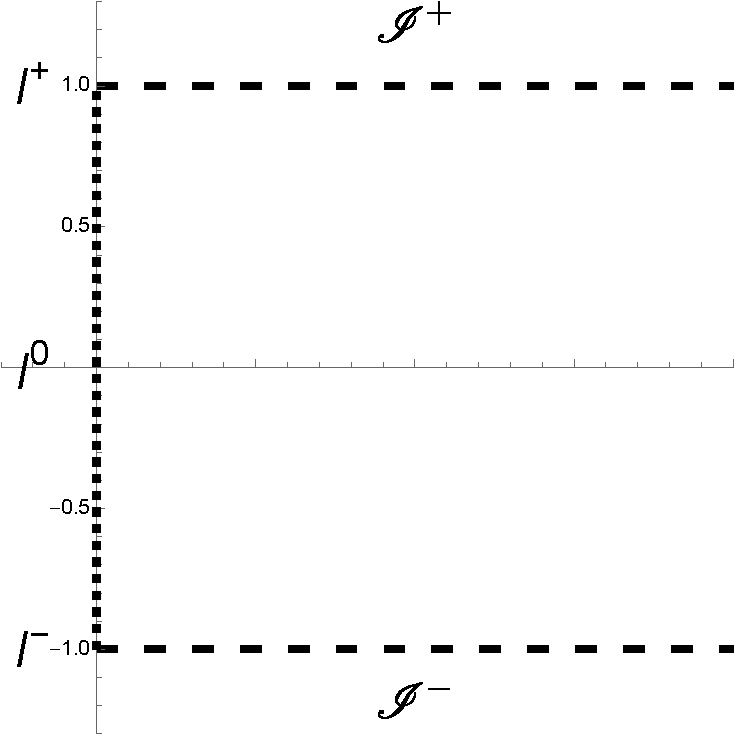
\includegraphics[width =0.35\textwidth]{friedrich cylinder.pdf}
    \caption{Representation of the Friedrich Cylinder. Past null infinity is represented by
    $\mathscr{I}^{-}$, Future null infinity $\mathscr{I}^{+}$, spatial infinity as $i^{0}$ and the critical sets as $I^{+}$ and $I^{-}$.}
\end{figure}

%%%%%%%%%%%%%%%%%%%%%%%%%%%%%%%%%%%%%%%%%%%%%%%%%%%%%%%%%%%%%%%%%%%%%%%%%%%%%%%%%%%%%%%%%%%%%%%%%%%%%%%%%%%%%%%%%%%%%%%%%%%%%%%%%%%%%%%%%%%%%%%%%%%%%%%%%%%%%%%%%%%%%
\section{Conclusions}
\label{sec:conclusions}

General relativity is a theory of gravitation that explains the force of gravity as a curvature of spacetime caused by mass and energy. Black holes, which are objects with such strong gravitational forces that nothing, not even light, can escape them, are an important aspect of this theory. When an object falls into a black hole, it is reduced to just three numbers, leading to the loss of a large amount of information, a problem known as the "information paradox." A recent theory called "soft hair" has been proposed to explain this paradox by positing that non-trivial distortions in clocks, sensitive to the black hole's consumption history, can provide an infinite number of properties for a black hole in certain limits. The Newman-Penrose (NP) constants are quantities defined on null infinity in general relativity that obey conservation laws for asymptotically flat gravitational fields. These constants can be used to study the residual radiation present in spacetime after a black hole collision, and have been shown to be zero for stationary spacetimes such as the Schwarzschild and Kerr solutions. However, it is still an open question whether the NP constants are zero for all stationary spacetimes. \\

In this thesis, we have computed the Newman-Penrose (NP) constants for a spin-0 field propagating near spatial and null infinity. The analysis was carried out using prescribed analytic initial data close to $i^0$ in Minkowski spacetime, and we discussed the infinite hierarchy of NP constants. \\

To achieve this, we employed the concept of the $i^0$ cylinder framework. We investigated the relation between the NP constants at future and past null infinity by identifying the specific part of the initial data that determines these constants. It was noted that when analytic initial data is prescribed near $i^0$, the solution loses regularity at the critical sets $\mathcal{I}^{\pm}$, where $i^0$ and $\mathscr{I}$ meet. This loss of regularity is governed by a constant $D_{p;p,m}$ present in the parametrization of the initial data. When the regularity condition ($D_{p;p,m} = 0$) is not satisfied, the classical NP constants are not well-defined. \\

However, in cases where the regularity condition is satisfied, we found that the classical NP constants at $\mathscr{I}^{\pm}$ arise from independent parts of the initial data. These parts are parametrized by the constants $A_{\ell+1;\ell,m}$ and $B_{\ell+1;\ell,m}$, respectively. As a result, there is no direct correspondence between the NP constants at future and past null infinity. \\

Nevertheless, we also showed that utilizing the $f(\tilde{\rho})$-modified NP constants proposed in \cite{Keh21_a}, with $f(\tilde{\rho})=\tilde{\rho}$, yields conserved quantities that do not require the regularity condition. In fact, these modified constants precisely correspond to the terms in the initial data that control the regularity of the field: $D_{p;p,m}$. This offers a valuable alternative approach to studying the conservation properties of the system without relying on the regularity condition. \\

In conclusion, it is evident that while the classical NP constants at $\mathscr{I}^{\pm}$ do not generally match, the \emph{$i^0$ cylinder NP constants} at $\mathscr{I}^{\pm}$ do coincide, up to a numerical factor. This remarkable alignment is a result of their origin from the same part of the initial data.


